
\documentclass[open=any]{SPhdThesis}

% Packages.
\usepackage{listings}
\usepackage{titlesec}
\usepackage{todonotes}
\usepackage[utf8]{inputenc}
\usepackage[english]{babel}
\usepackage{amsthm}
\usepackage[titletoc]{appendix}

% Environments
\newtheorem{theorem}{Theorem}[section]
\newtheorem{corollary}{Corollary}[theorem]
\newtheorem{lemma}[theorem]{Lemma}
\newtheorem{partconclusion}{Partial Conclusion}[chapter]
\newtheorem{definition}{Definition}[chapter]
\newtheorem{researchquestion}{Research Question}
\newtheorem{scenario}{Scenario}

% PDF and title properties.
\SgSetTitle{Automatic generation of multi-language object domain models through a Shape Expressions subset}
\SgSetAuthor{Guillermo Facundo Colunga}
\SgSetAuthorDegrees{}
\SgSetYear{2020}
\SgSetDegree{Software Engineer}
\SgSetDepartment{Department of Computer Science}
\SgSetUniversity{University of Oviedo}
\SgSetDeclarationDate{July 2020}

% The document.
\begin{document}
	\begin{frontmatter}
		\SgAddTitle%
		%\SgAddDeclaration%
		\begin{acknowledgments}
    This work has been partially funded by the European
    Hercules project through the WESO research group at
    the University of Oviedo.

    In addition, for the development of the research we
    have worked with different research groups and researchers
    such as Dublin Core or Eric Prud'hommeaux to whom I would
    like to thank the warm welcome.

    Finally, I would like to thank my tutors Jose Emilio
    Labra Gayo and Daniel Fernández Álvarez for all the
    work carried out within the framework of this project.

\end{acknowledgments}%
		\begin{abstract}
Surface integration is an important step for automatic 3D reconstruction of real objects.
The goal of a surface integration algorithm is to reconstruct a surface from a set of range
images registered in a common coordinate system. Based on the surface representation used,
existing algorithms can be divided into two categories: volume-based and mesh-based.
Volume-based methods have been shown to be robust to scanner noise and small features
(regions of high curvature) and can build water tight models of high quality. It is, however,
difficult to choose the appropriate voxel size when the input range images have both small
features and large registration errors compared to the sampling density of range images.
Mesh-based methods are more efficient and need less memory compared to volume-based methods
but these methods fail in the presence of small features and are not robust to scanning noise.

This paper presents a robust algorithm for mesh-based surface integration of a set of range
images. The algorithm is incremental and operates on a range image and the model reconstructed
so far. Our algorithm first, transform the model in the coordinate system of the range image.
Then, it finds the regions of model overlapping with the range image. This is done by shooting
rays from the scanner, through the vertices in the range image and intersecting them with the
model. Finally, the algorithm integrates the overlapping regions by using weighted average of
points in the model and the  range image. The weights are computed using the scanner uncertainty
and helps in reducing the effects of scanning noise. To handle small features robustly the
integration of overlapping regions is done by computing the position of vertices in the range
image along the scanner's line of sight. Since for every point in a range image there is exactly
one depth value, the reconstructed surface in the regions of high curvature will not have
self-intersections.

\bigskip
\textbf{Keywords ---} \textit{RDF, Linked Data, RDF Validation, Shape Expressions, Lexical-Sintactic and
Semantic Validator, Object Oriented Programming Languages, Compiler, Translator.}
\end{abstract}%
		\SgAddToc%  Table of contents.
		\SgAddLof%  List of figures.
		\SgAddLot%  List of tables.
		%\SgAddLoa%  List of algorithms.
	\end{frontmatter}
   
	\chapter{Introduction}
\label{ch:intro}

This chapter covers the motivation, contributions and structure of the document.
The main objective of this chapter, therefore, is that after reading it, the reader
builds an idea about the motivations that have promoted this project, what is
being worked on and the contributions emanating from it.

% S E C T I O N   M O T I V A T I O N

\section{Motivation}
\label{sec:intro-motiv}

Each day, more and more devices generate data both automatically and manually, and also each day the development of
applications in different domains that are backed by databases and expose these data to the web becomes easier. The
amount and diversity of data produced clearly exceeds our capacity to consume it.

To describe the data that is so large and complex that traditional data processing applications can’t handle the
term Big Data \cite{big-data,sagiroglu2013big} has emerged. Big Data has been described by at least three words starting
by V: volume, velocity, variety. Although volume and velocity are the most visible features, variety is a key concept
which prevents data integration and generates lots of interoperability problems.

RDF \textit{(Resource Description Framework)} was proposed as a graph-based data model
\cite{graph-data-model} which became part of the Semantic Web \cite{semantic-web} vision.
Its reliance on the global nature of URIs\footnote{A Uniform Resource Identifier (URI) is a string of
characters that unambiguously identifies a particular resource. To guarantee uniformity, all URIs follow a predefined
set of syntax rules, but also maintain extensibility through a separately defined hierarchical naming scheme.
Ref.\url{https://en.wikipedia.org/wiki/Uniform_Resource_Identifier}} offered a solution to the data integration
problem as RDF datasets produced by different means can seamlessly be integrated with other data.

Related to this, is the concept of Linked Data \cite{linked-data} that was proposed as a set of best
practices to publish data on the Web. It was introduced by Tim Berners-Lee and was based on four main principles,
as mentioned in \cite{linked-data}:

\begin{itemize}
  \item Use URIs as names for things.
  \item Use HTTP URIs so that people can look up those names.
  \item When someone looks up a URI, provide useful information, using the standards (RDF, SPARQL).
  \item Include links to other URIs. so that they can discover more things.
\end{itemize}

\begin{figure}
    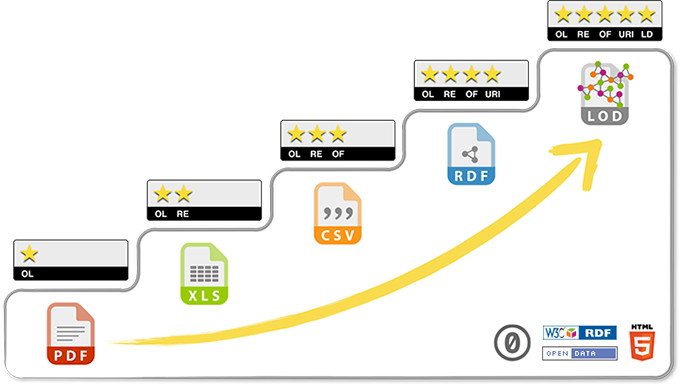
\includegraphics[scale=0.5]{images/5-star-steps.png}
    \centering
	\caption[The 5 star steps of Linked Data]{The 5 star steps of Linked Data.}
	\label{fig:margin-5-star-steps}
\end{figure}

Similar to this four principles is the 5 stars Linked Open Data Model, illustrated in \cref{fig:margin-5-star-steps}.
RDF is mentioned in the third principle as one of the standards that provides useful information. The goal of this
principles is that data is not only ready for humans to navigate through but also for other agents, like computers,
that may automatically process that data.

All the above motivations helped to make RDF the language for the Web of Data, as described in \cite{labra-validating-rdf}.
And the main features that it presents are: \textit{Disambiguation}, \textit{Integration}, \textit{Extensibility}, \textit{Flexibility} and \textit{Open by Default}.
With the features also some drawbacks are associated, the most important one and the one we will focus is the RDF
\textbf{production/consumption dilemma}.

RDF production/consumption dilemma states that it is necessary to find ways that data producers can generate their data so
it can be handled by potential consumers. For example, they may want to declare that some nodes have some properties with
some specific values. Data consumers need to know that structure to develop applications to consume the data.

Although RDF is a very flexible schema-less language, enterprise and industrial applications may require an extra level of
validation before processing for several reasons like security, performance, etc.

To solve that dilemma and as an alternative to expecting the data to have some structure without validation, Shape Expressions Language
\textit{(ShEx)} was proposed as a human-readable and high-level open source language for RDF validation. Initially, ShEx was proposed
as a human-readable syntax for OSLC Resource Shapes \cite{oslc-resource-shape} but ShEx grew very fast to embrace more
complex user requirements coming from clinical and library use cases.

Another technology, SPARQL Inferencing Notation (SPIN) \cite{knublauch2011spin}, was used for RDF validation, principally in TopQuadrant’s TopBraid Composer. This technology, influenced
from OSLC Resource Shapes as well, evolved into both a private implementation and open source definition of the SHACL
\textit{(Shapes Constraint Language)}, which was adopted by the W3C Data Shapes Working Group.

From a user point of view the possibilities of ShEx are very large, from the smallest case to just validate a node with one property
to a scientific domain case where we need to validate the human genome\footnote{\url{https://github.com/geneontology/go-shapes}}. A language with such a number
of possibilities requires from a strong syntactic and semantic validation and that leads us to our first goal.

\begin{researchquestion}
  Determine how much the existing syntactic and semantic validation systems for shape expressions can be enhanced. And
  if existing systems can be enhanced propose a prototype that implement those enhancements.
\end{researchquestion}

Secondly and very related to programming languages, if we take the PopularitY of Programming Language \textit{(PYPL)} Index\footnote{\url{http://pypl.github.io/PYPL.html}}
from June 2020 we can see that more than half of the share is occupied by languages that support the object oriented paradigm. And therefore this paradigm
becomes the most used one. The aim of this paradigm is to model real world domains, according to \cite{wegner1990concepts}. That, in fact, is the same goal
that ShEx has, it allows to model real world domains with schemas, and validate existing data with them. Therefore our second goal relies on this and tries
to automatically transform shape expressions into object domain models coded in any language that supports the object oriented paradigm:

\begin{researchquestion}
  Determine till which point can we automatically translate existing shape expressions to object domain models. And
  propose a prototype capable of translating Shape Expressions to object domain models.
\end{researchquestion}

If this were possible it would not only imply that you could automate the creation of application domain models but that you could link the domain model that an
application uses with a domain model defined through Shape Expressions that describes the schema of a RDF data set.

\bigskip

To give answers to the questions posed in this section, we will limit our scope to the micro grammar of Shape Expressions, defined in
\footnote{\url{https://dcmi.github.io/dcap/shex_lite/micro-spec.html}}. This version is a strict subset of the complete ShEx grammar
and therefore any derived method or technology we can draw from it can automatically be applied to the full grammar.

% S E C T I O N   C O N T R I B U T I O N S

\section{Contributions}
\label{sec:intro-contri}
These are the major contributions of this dissertation:

\begin{enumerate}
  \item A parser for the ShEx micro Compact Syntax. There are already existing parsers for ShEx and they work for ShEx micro Compact Syntax
  as it is a subset of ShEx, but they accept more structures than the ones defined by ShEx micro Compact Syntax. We propose a parser that
  is only focused on ShEx micro Compact Syntax and therefore error and warning messages can be enhanced.
  
  \item Error and warning analyser for schemas. Existing approaches do not semantically validate the schemas, they
  only perform error detection by means of complex grammars and parsers. Our proposed system does semantically validate the schemas by means
  of a custom analyser that performs both syntactic and semantic analysis so it produces human-friendly errors and warnings that users can
  use to fix their schemas.

  \item Automatic translation of schemas into object domain models in \texttt{Java} and \texttt{Python}. The proposed system
  integrates an open back-end with built-in code translation from the validated schemas to domain models in Object
  Oriented Programming Languages \textit{(OOPL)} \cite{oopl}.

  \item Evaluation of errors and warnings generated of our proposed solution against existing tools. This comparison
  empirically shows the benefits and drawbacks of our proposed system.
\end{enumerate}

% S E C T I O N   S T R U C T U R E   O F   T H E   D O C U M E N T

\section{Structure of the Document}
\label{sec:intro-structure}
The dissertation layout is as follows:
\bigskip

\begin{description}
  \item[\cref{ch:theo-back}] Indicates the state of the art of the existing RDF validation technologies, tools for processing Shape
  Expressions and other related projects.
	\item[\cref{ch:retalted-work}] Gives a basic theoretical background that it is needed to fully understand the concepts explained in the
  following chapters.
  \item[\cref{ch:current-analysers-analysis}] Analyses current syntactic and semantic analysis systems.
  \item[\cref{ch:proposed-sin-sema-anal}] He proposes a system by means of software engineering techniques
  that tries to solve the problem posed in the previous chapter.
  \item[\cref{ch:proposed-implementation}] It proposes an implementation that meets the expectations of the previous chapter.
  This implementation is the one that will be used to carry out the evaluation of results.
  \item[\cref{ch:odm-transl}] Define the ShEx translation problem to object-oriented languages and compare the
  expressivities of both systems.
  \item[\cref{ch:proposed-translator}] It focuses on proposing a solution to the problem raised in the previous chapter.
  First through formalizations and then employing software engineering methodologies.
  \item[\cref{ch:proposed-system}] It offers a proposed implementation to meet the expectations of the previous chapters.
  This implementation will be used to evaluate the results.
  \item[\cref{ch:results-evaluation}] It defines a methodology and the data on which the methodology will be tested. Then evaluate the results obtained.
  \item[\cref{ch:planning-and-budget}] It includes the description of the project planning as well as its cost budget.
  \item[\cref{ch:conclusions}] It summarizes the results achieved after completing the work and includes the proposals for future work.
\end{description}
	\chapter{Teoretical Background}
\label{ch:theo-back}

For a proper understanding of this documentation and the ideas explained on it it is
needed to know some theoretical concepts that are the fundaments of Linked Data, RDF,
RDF Validation, programing languages and compilers. This sections is devoted to carefully
explain those concepts to the needed deepth to fully understand this dissertation, but for
those readers that want a deeper explanation a more detailed view of the concepts
presented here is offered in \cite{labra-validating-rdf, eric-rdf-validation-lang,
programing-language}.

% S E C T I O N   R D F

\section{RDF}
\label{sec:theo-back-rdf}
Resource Description Framework (RDF) is a standard model for data interchange on the web,
started in 1998 and the first version of the specification was published in 2004 by the W3C
according to \cite{rdf-primer}. RDF has features that facilitate data merging even if the
underlying schemas differ, and it specifically supports the evolution of schemas over time
without requiring all the data consumers to be changed. Another important feature is that RDF
supports XML, N-Triples and Turtle syntax, the \cref{fig:rdf-ntriples-ex} shows an example of
how a triplet can be written in RDF N-Triples Syntax.

\begin{figure}
\begin{lstlisting}[numbers=left, basicstyle=\ttfamily\scriptsize]
<http://example/subject1> <http://example/predicate1> <http://example/object1> .
\end{lstlisting}
\caption[RDF N-Triples Example]{RDF N-Triples Example. From this example we can see that each triplet is
composed of three elements, the subject the predicate and the object.}
\label{fig:rdf-ntriples-ex}
\end{figure}

RDF extends the linking structure of the Web to use URIs to name the relationship between
things as well as the two ends of the link (this is usually referred to as a “triple” or "triplet").
Using this simple model, it allows structured and semi-structured data to be mixed, exposed,
and shared across different applications. \ref{fig:rdf-graph} shows an example of how different
triples can be use to compose a graph, this graph represents the same as the \cref{fig:rdf-ntriples-graph}

\begin{figure}
\begin{lstlisting}[numbers=left, basicstyle=\ttfamily\scriptsize]
<http://example/bob> <http://example/knows> <http://example/alice> .
<http://example/alice> <http://example/knows> <http://example/peter> .
\end{lstlisting}
\caption[RDF N-Triples Graph Example]{RDF N-Triples Graph Example. This exmaple shows the n-triples
that generate the graph from \cref{fig:rdf-graph}.}
\label{fig:rdf-ntriples-graph}
\end{figure}

This linking structure forms a directed, labeled graph, where the edges represent the named link
between two resources, represented by the graph nodes. This graph view is the easiest possible
mental model for RDF and is often used in easy-to-understand visual explanations.

Also, related to this we strongly recommend the Tim Berners-Lee’s writings on Web Design Issues
\cite{semantic-roadmap} where he explain the issues of the liked data and why is RDF so important.

\begin{figure}
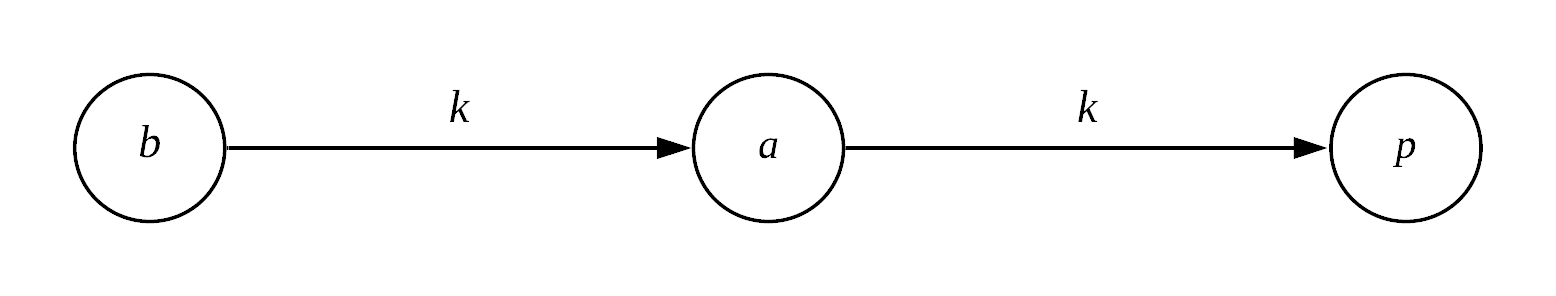
\includegraphics[scale=0.2]{images/shex-lite-rdf-graph.png}
\centering
\caption[RDF Example graph]{RDF graph formed by triplets from \cref{fig:rdf-ntriples-graph}, where
\textit{b} corresponds to \textit{\texttt{<http://example/bob>}}, \textit{a} corresponds to
\textit{\texttt{<http://example/alice>}}, \textit{p} corresponds to \textit{\texttt{<http://example/peter>}}
and \textit{k} corresponds to \textit{\texttt{<http://example/knows>}}.}
\label{fig:rdf-graph}
\end{figure}

% S E C T I O N   V A L I D A T I N G   R D F

\section{Validating RDF}
RDF therefore allows to represent and store data, and with this ability emerges the need to validate
that the schema of the graph is correct. In order to perform the validation of RDF data there  have
been previous attempts, described in \cref{sec:aaa}, this dissertation will focus
on Shape Expressions. But in order to validate RDF data every technology will need to face the following
RDF concepts:

\begin{itemize}
 \item the form of a node (the mechanisms for doing this will be called “node constraints”);
 \item the number of possible arcs incoming/outgoing from a node; and
 \item the possible values associated with those arcs.
\end{itemize}

\begin{figure}
  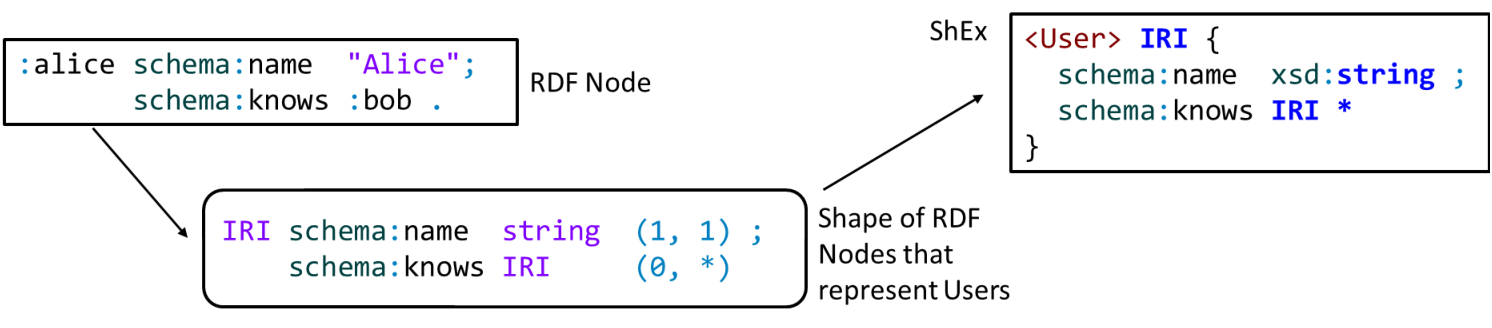
\includegraphics[scale=0.25]{images/rdf-node-and-shape.png}
  \centering
  \caption[RDF node and its shape]{RDF node and its shape.}
  \label{fig:rdf-graph-2}
\end{figure}

\cref{fig:rdf-graph} illustrates those RDF concepts by means of the Shape Expression that validates users.
There we can see that the shape of the RDF node that represents Users represents the form of a node,
the number of possible arcs and the possible value associated with those arcs.

\subsection{Shape Expressions}
As defined in \cite{labra-validating-rdf} Shape Expressions (ShEx) is a schema language for describing RDF
graphs structures. ShEx was originally developed in late 2013 to provide a human-readable syntax for OSLC
Resource Shapes. It added disjunctions, so it was more expressive than Resource Shapes. Tokens in the language
were adopted from Turtle and SPARQL with tokens for grouping, repetition and wildcards from regular expression
and RelaxNG Compact Syntax \cite{van2003relax}. The language was described in a paper
\cite{eric-rdf-validation-lang} and codified in a June 2014 W3C member submission which included a primer and
a semantics specification. This was later deemed “ShEx 1.0”.

As of publication, the ShEx Community Group was starting work on ShEx 2.1 to add features like value comparison
and unique keys. See the ShEx Homepage \url{http://shex.io/} for the state of the art in ShEx. A collection of
ShEx schemas has also been started at \url{https://github.com/shexSpec/schemas}.

\begin{figure}
\begin{lstlisting}[numbers=left, basicstyle=\ttfamily\scriptsize]
PREFIX :       <http://example.org/>
PREFIX schema: <http://schema.org/>
PREFIX xsd:  <http://www.w3.org/2001/XMLSchema#>

:User {
  schema:name          xsd:string  ;
  schema:birthDate     xsd:date?  ;
  schema:gender        [ schema:Male schema:Female ] OR xsd:string ;
  schema:knows         IRI @:User*
}
\end{lstlisting}
\caption[Shape Expression Example]{Shape Expression Example. This example describes a shape expression that
describes a user as a node that has one name of type string, an optional bithd date of type date, one gende
of type Male, Female or free string and a set between 0 and infinite of other users represented by the knows
property.}
\label{fig:shape-expr-ex}
\end{figure}

\subsubsection{ShEx Compact Syntax: \texttt{ShExC}}
The ShEx compact syntax (ShExC) was designed to be read and edited by humans. It follows some conventions which
are similar to Turtle or SPARQL.

\begin{itemize}
    \item \texttt{PREFIX} and \texttt{BASE} declarations follow the same convention as in Turtle. In the rest of
    this chapter we will omit prefix declarations for brevity.
	\item Comments start with a \texttt{\#} and continue until the end of line.
	\item The keyword a identifies the \texttt{rdf:type} property.
    \item Relative and absolute IRIs are enclosed by \texttt{< >} and prefixed names (a shorter way to write
    out IRIs) are written with prefix followed by a colon.
	\item Blank nodes are identified using \texttt{\_:label} notation.
    \item Literals can be enclosed by the same quotation conventions ( \texttt{'}, \texttt{"}, \texttt{'''},
    \texttt{"""}) as in Turtle.
    \item Keywords (apart from a) are not case sensitive. Which means that \texttt{MinInclusive} is the same
    as \texttt{MININCLUSIVE}.
\end{itemize}

A ShExC document declares a ShEx schema. A ShEx schema is a set of labeled shape expressions which are composed
of node constraints and shapes. These constrain the permissible values or graph structure around a node in an RDF
graph. When we are considering a specific node, we call that node the focus node.

\begin{figure}
  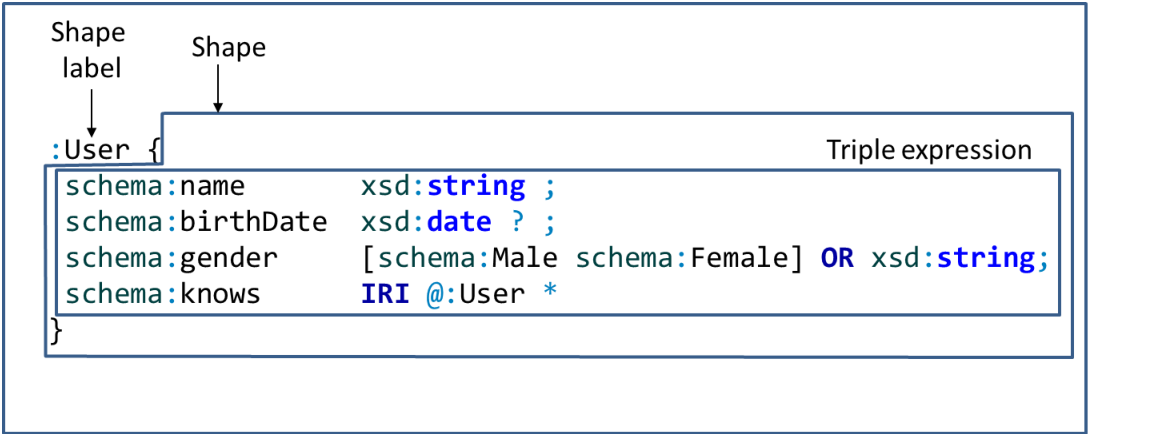
\includegraphics[scale=0.25]{images/shex-out.png}
  \centering
  \caption[Shapes, shape expression labels and triple expressions]{Shapes, shape expression labels and triple expressions.}
  \label{fig:shex-out-view}
\end{figure}

\cref{fig:shex-out-view} shows the first level of a shape expression, we have a label and the shape itself that is
what we asing to the \texttt{:User} label. Then, the shape is composed by triple expressions. The triple expression
structure is explained in \cref{fig:shex-triple-expression}, and as its name indicates it is composed of three
elements, the property, the node constraint and the cardinality.

\begin{figure}
  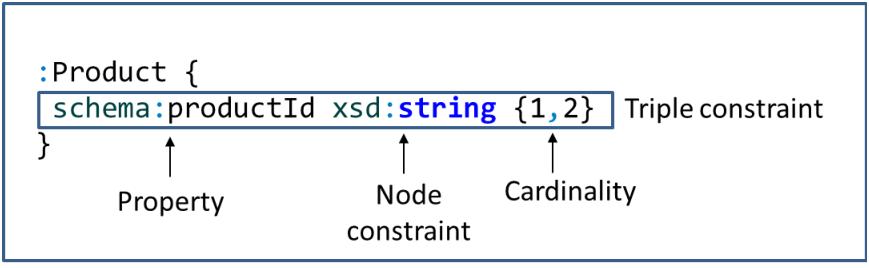
\includegraphics[scale=0.25]{images/shex-triple-expression.png}
  \centering
  \caption[Parts of a triple expression]{Parts of a triple expression.}
  \label{shex-triple-expression}
\end{figure}

Shape Expressions Compact Syntax is much bigger and containts other multiple features that give ShEx its power,
and all of them can be explored in \cite{labra-validating-rdf} but they are not needed to understand this
dissertation.

\subsubsection{Use of ShEx}
Strictly speaking, a ShEx schema defines a set of graphs. This can be used for many purposes, including
communicating data structures associated with some process or interface, generating or validating data,
or driving user interface generation and navigation. At the core of all of these use cases is the notion
of conformance with schema. Even one is using ShEx to create forms, the goal is to accept and present
data which is valid with respect to a schema. ShEx has several serialization formats:

\begin{itemize}
	\item a concise, human-readable compact syntax (ShExC);
	\item a JSON-LD syntax (ShExJ) which serves as an abstract syntax; and
	\item an RDF representation (ShExR) derived from the JSON-LD syntax.
\end{itemize}

These are all isomorphic and most implementations can map from one to another.
Tools that derive schemas by inspection or translate them from other schema languages typically generate ShExJ.
Interactions with users, e.g., in specifications are almost always in the compact syntax ShExC. As a practical
example, in HL7 FHIR, ShExJ schemas are automatically generated from other formats, and presented to the end
user using compact syntax.

ShExR allows to use RDF tools to manage schemas, e.g., doing a SPARQL query to find out whether an organization
is using dc:creator with a string, a foaf:Person, or even whether an organization is consistent about it.

\subsubsection{ShEx Implementations} \todo{Check links.}
At the time of this writing, we are aware of the following implementations of ShEx.

\begin{itemize}
	\item shex.js for Javascript/N3.js (Eric Prud’hommeaux) \url{https://github.com/shexSpec/shex.js/};
	\item Shaclex for Scala/Jena (Jose Emilio Labra Gayo) \url{https://github.com/labra/shaclex/};
	\item shex.rb for Ruby/RDF.rb (Gregg Kellogg) \url{https://github.com/ruby-rdf/shex};
	\item Java ShEx for Java/Jena (Iovka Boneva/University of Lille) \url{https://gforge.inria.fr/projects/shex-impl/}; and
	\item ShExkell for Haskell (Sergio Iván Franco and Weso Research Group) \url{https://github.com/weso/shexkell}.
\end{itemize}

There are also several online demos and tools that can be used to experiment with ShEx.

\begin{itemize}
	\item shex.js (http://rawgit.com/shexSpec/shex.js/master/doc/shex-simple.html);
	\item Shaclex (http://shaclex.herokuapp.com); and
	\item ShExValidata (for ShEx 1.0) (https://www.w3.org/2015/03/ShExValidata/).
\end{itemize}

\subsection{Other Technologies}
\label{subs:theo-back-validating-other-techs}
As other validation technologies we will just explore the existence of them as it is very interesting to know how
other tools approach the same issue.

\subsubsection{SHACL}
Also in \cite{labra-validating-rdf}, Chapter 5, it is fully explained that Shapes Constraint Language (SHACL)
has been developed by the W3C RDF Data Shapes Working Group, which was chartered in 2014 with the goal to “produce
a language for defining structural constraints on RDF graphs \cite{oslc-resource-shape}.”

The main difference that made us choose ShEx over SHACL are that ShEx emphasized human readability, with a
compact grammar that follows traditional language design principles and a compact syntax evolved from Turtle.

\subsubsection{JSON Schema}
JSON Schema born as a way to validate JSON-LD, and as turtle and RDF can be serialized as JSON-LD it is usual to
think that JSON Schema can validate RDF data, but this is not fully correct. And the reason is that the serialization
of RDF data in to JSON-LD is not deterministic, that means that a single schema might have multiple serializations,
which interferes with the validation as you cannot define a relative schema.

% S E C T I O N   P R O G R A M M I N G   L A N G U A G E S

\section{Programming Languages}
According to \cite{programing-language} “a programming language is a formal language comprising a set of instructions
that produce various kinds of output.” When we talk about programming languages we need to know that they are split into
two, General Purpose Languages (GPL) and Domain Specific Languages (DSL). The main difference overtime is that, as said
in \cite{dsl}, a domain-specific language (DSL) is a computer language specialized to a particular application domain
in contrast to a general-purpose language (GPL), which is broadly applicable across domains.

In the specific case of ShEx-Lite we will be talking about a Domain Specific Language, and more deep we would classified
it as a Declarative one, that means that it is not Touring Complete \cite{touring-complete}.

% S E C T I O N   C O M P I L E R S

\section{Compilers}
A compiler is a computer program that translates computer code written in one programming language (the source language)
into another language (the target language). Is during this translation process where the compiler validates the syntax
and the semantics of the program, if any error is detected in the process the compiler raises an exception (understand
as a compiler event that avoids the compiler to continue its execution).

\subsection{Internal Structure}
In order to decompose the internal structure of a compiler they have been split in to the most common task they do
\cref{fig:compiler-stages}, of course this doesn’t mean that there are compilers with more or less stages, but at the
end everything can be group into any of the groups that we will explain:

\begin{figure}
  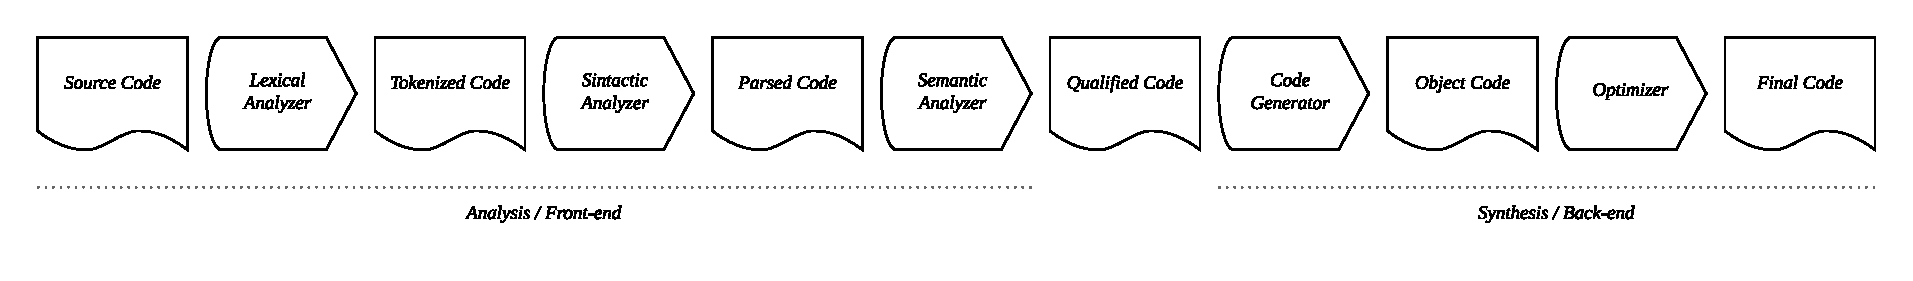
\includegraphics[width=\textwidth]{images/compiler-stages.pdf}
  \centering
  \caption[Compiler stages]{Compiler stages.}
  \label{fig:compiler-stages}
\end{figure}

\subsubsection{Lexycal Analyzer}
The lexical analyzer task is to get the input and split it in to tokens \cite{lexical-analysis}, which are build
from lexemes. If the compiler cannot find a valid token for some lexemes in the source code will generate an error,
as the input cannot be recognized.

\subsubsection{Syntactic Analyzer}
The syntactic analyzer takes the tokens generated during the lexical analysis and parses them in such a way that try’s
to group tokens so the conform to the language grammar rules. During this stage if there is any error while trying to
group the tokens then the compiler will rise an error as the input cannot be parsed.

\subsubsection{Semantic Analyzer}
The semantic analyzer has two main tasks, usually. First it validates that the source code semantics are correct, for
example 4 + “aaa” would not make sense. And the second task is to transform the Abstract Syntax Tree in to a type-checked
and annotated AST. Usually that means relate the invocations and variables to its definition, very useful for type-checking.

\subsubsection{Code Generator}
The task of the code generator as its name indicates is to generate the target code, it can be byte code, machine code
or even another high-language code.

\subsubsection{Code Optimizer}
The code optimizer is the last step before the final target code is generated, it rewrites the code that the code generator
produced without changing the semantics of the program, its aim is just to make code faster. At \cite{compiler-optimizations}
you can see an example of some optimizations that can be done at compile time to make your code faster.

\subsection{Conventional Compilers}
Conventional compiler are a big monolith where each stage \ref{fig:compiler-stages} is executed automatically after the
previous stage, if the compiler has eight steps you need to execute them all at once. This approach have been the “old-fashion”
but it presents some drawbacks:
\begin{itemize}
    \item A poor IDE \cite{ide} integration. IDE’s need to perform incremental compilations in matter of nanoseconds so
    the user doesn’t feel lag when typing the program. With conventional compilers as you need to go through all the compilation
    process at once they where very slow and companies like Microsoft need to develop different compilers, one for the IDE and
    another for the final compilation of the program itself. This lead to several problems like that if a feature gets
    implemented in the final compilation compiler but not in the IDE one the IDE would not support the feature meanwhile
    the language would.
    \item Difficult to debug. As the conventional compilers where a blackbox the only way to test intermediate stages was
    by throwing an input and waiting the the feature you wanted to test was thrown for that input.
\end{itemize}

\subsection{Modern Compilers}
After the problems Microsoft had with the C\# compiler they decide to rewrite the whole compiler and introduce a concept
called “compiler as an API” with Roslyn \cite{dotNet}. This concept has been perfectly accepted and solved many problems.
In this concept each stage has an input and an output that can be accessed from outside the compiler and stages can be
executed independently on demand. This means that for example if an IDE just want to execute the Lexer the Parser and
the Semantic analysis it can. That translates in to speed for the user.

Also the second problem is solved as testing individual parts of the compiler is much more easy than the hole compiler
at once.

	\chapter{Related Work}
\label{ch:retalted-work}

Some work has already been done in the field of Shape Expressions and RDF validation
technologies. In this chapter we will go over the main studies related to our project,
exploring what they have achieved and some of their limitations.

% S E C T I O N   S I M P L I F I C A T I O N S   O F   S H E X

\section{Simplifications of ShEx}
\label{sec:related-work-simplifications}

\subsection{The \textbf{S} language}

In 2019 at \cite{rdf-challenges} was defined a language called \textbf{S} as a simple abstract
language that captures both the essence of ShEx and SHACL. This is very relevant as this language
is intended to be the input of a theoretical abstract machine that will be used for graph validation
for both ShEx and SHACL. Also in the same paper the authors carefully describe the algorithm for the
translation from ShEx to S and from SHACL to S.

Although the theoretical abstract machine has not been implemented yet the intention of the WESO
Research Group, where this S language was defined, is to devote more efforts in to this project
during the 2021.

Other definition of an abstract language based on uniform schemas can be found at \cite{iovka-auto-shex-shacl}.
This language is focused on schemas inference rather on validation, but needs to be taken
into account as they also perform an abstraction of both ShEx and SHACL.

\subsection{ShExJ Micro Spec}
Recently the Dublin Core Team\footnote{\url{https://dublincore.org/}} is working into an
specification that allows to define Shape Expressions in tabular formats. For this specification
they propose a simplification of the Shape Expressions JSON syntax that allows to define an
schema as a set of simple triple constraints. This specification is not official and has
not been validated yet but it is very important for our work as we will also work in a
simplification of a syntax of ShEx.

\bigskip

And to the best of our knowledge and after the research process carried out for this
project no other language based on a subset of Shape Expressions has been designed nor implemented yet.

% S E C T I O N   S H E X   E C O S Y S T E M

\section{ShEx Ecosystem Tools}
\label{sec:related-work-shex-ecosystem}

We already know that ShEx and SHACL have been the two main technologies for RDF validation and some tools
emerged around them, we thinks that some of them might benefit from ShEx-Lite. Here we introduce briefly
those that had the biggest impact in the community.

\subsection{Validators}
Since the beginning of ShEx and SHACL as languages the RDF community started to build tools that take as
input the schemas defined and validate graphs.

This kind of tools can benefit from SHEx-Lite from the point of view that new functionalities can be easily
implemented and tested in the lite version of the language before even touching the stable releases of both
tools. In the case of ShEx this is more obvious as ShEx-Lite and ShEx are both implemented in Scala and if
good design principles are used functionalities can be just migrated and expanded for the rest of the language.

The most important validators are:

\subsubsection{Shaclex}
According to the Shaclex\footnote{\url{https://github.com/weso/shaclex}} official website it is an Open
Source Scala pure functional implementation of an RDF Validator that supports both Shape Expressions and
SHACL. It was initially developed by Dr. Jose Emilio Labra Gayo and is being maintained by an active
community on GitHub. It is used by different projects around the globe and its goal is to validate RDF
graphs against schemas defined in Shape Expression or in SHACL.

This implementation of a ShEx validator is very important for us as ShEx-Lite is completely inspired by it
and aims to transfer the syntactic an semantic validation enhancements to it.

\subsubsection{ShEx.js}
Another example of a ShEx validator implementation is \texttt{ShEx.js} which is JavaScript based and also
open source on GitHub. This implementation is very important for the ShEx community as they defined the
serialization of the AST in this implementation as the abstract syntax of ShEx.


\subsection{IDEs}
In order to facilitate the task of writing schemas some engineers decide to implement specific IDEs for the
Shape Expressions Language.

This tools will completely benefit from ShEx-Lite and there are currently collaborations in process. At the
time they work with Shaclex, which is structured as a conventional compiler, but with the API architecture
of ShEx-Lite IDEs can access directly to the syntactic and semantic modules so features like advances colouring
syntax or incremental compilation are available.

\subsubsection{YASHE}
YASHE\footnote{\url{https://github.com/weso/YASHE}} (Yet Another ShEx Editor), is a Shape Expressions IDE
which started as a fork ofYASQE(which is based on SPARQL). This tool performs lexical and syntactic analysis
of the content of the editor, thus offering the user a real-time syntactic error detector. It has features
like: syntax highlighting, visual aid elements (tooltips) and autocomplete mechanisms. In addition, it offers
a simple way of integrating into other projects.

\subsubsection{Protégé}
Protégé is a piece of software developed by the University of Stanford focused on ontology edition. During the
last year they added support for Shape Expressions edition on their own software so they became another ShEx IDE.

\subsubsection{VSCode}
VSCode is a source code light-weight editor developed by Microsoft and supported by Linux, macOS and Windows.
By default this editor does not support any programming language, the way it works is with packages that the
community develops and extends the functionality. One of those packages adds support for Shape Expressions
Compact syntax and transforms VSCode into a ShEx IDE.

This plugin does not add semantic validation and it is a clear target to benefit from ShEx-Lite features.

\subsection{Others}
Other researches focused their efforts in to inferring schemas to existing data sets and creating tools to that
evolved from ShEx in order to transform existing data.

\subsubsection{Shexer}
Shexer\footnote{\url{https://github.com/DaniFdezAlvarez/shexer}} is a python library aimed to perform automatic
automatic extraction of schemas in both ShEx and SHACL from an RDF input graph. That is if all the other tools
take the schemas as the input and validate a graph with it, this tool takes a graph and from it it infers the
schemas that it might contain. Its work is fully described in \cite{iovka-auto-shex-shacl, fernandez2016inference}.

\subsubsection{ShExML}
ShExML\footnote{\url{https://github.com/herminiogg/ShExML}} is a language based on ShEx (not a simplification nor
an abstraction of ShEx) that can map and merge heterogeneous data formats into a single RDF representation.
The main idea behind this tool is written at \cite{shexml}.

\bigskip

An example of how this different tools can work together thanks to ShEx-Lite would be the following, illustrated
at \cref{fig:shex-lite-shexer-integration}.
Wikidata currently holds millions of registers that do not have any schema that validates them. And they need to
make consumer that represents the data in to an object domain model. Without any tool this is just almost impossible,
but this shexer you can infer the schemas to ShEx-Lite syntax and with the ShEx-Lite compiler you can automatically
create the object domain model in your favourite OOL.

\begin{figure}
    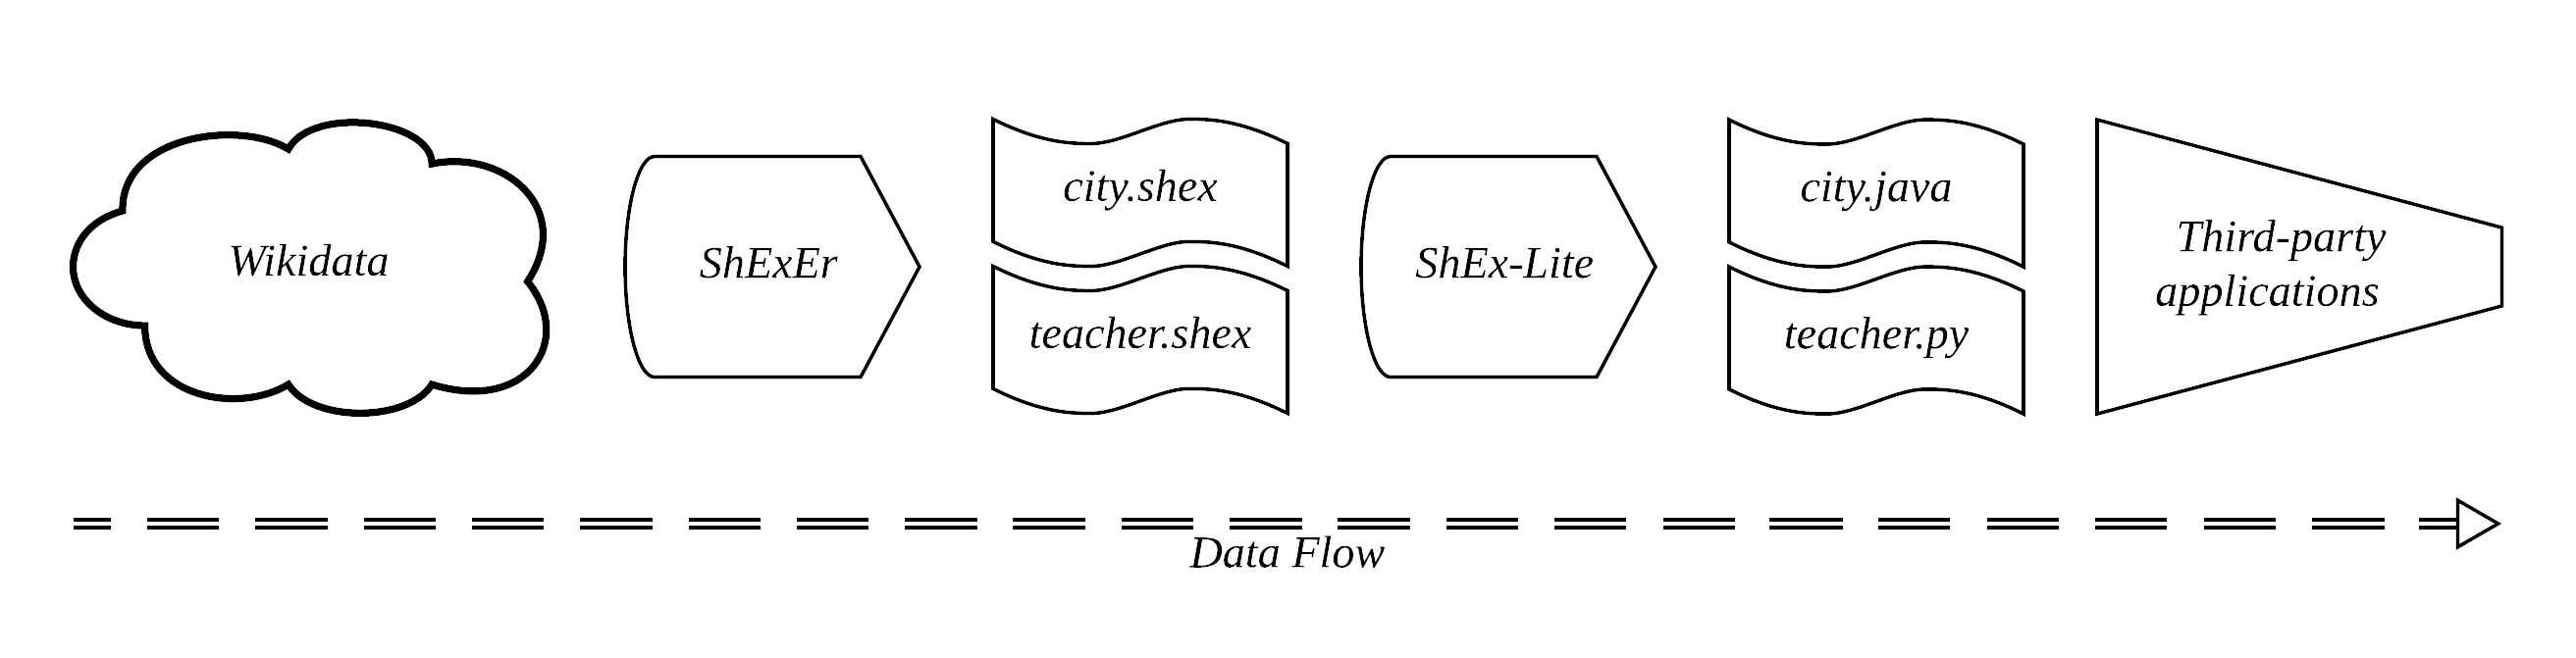
\includegraphics[width=\textwidth]{images/shex-lite-shexer-integration.png}
    \centering
    \caption[ShEx-Lite integration with Shexer]{ShEx-Lite integration with Shexer for automatically generating
    java domain object models for the Wikidata schema less existing data. This shoes the schema less data from
    wikidata from which shape expressions are inferred by shexer and later transformed to java plain objects by
    means of ShEx-Lite so third party applications can implement the domain model.}
	\label{fig:shex-lite-shexer-integration}
\end{figure}

	\part{Enhancing Error and Warning Detection and Emition on ShEx}
	\chapter{Analysis of Existing Sintactic and Semantic Analizers}
\label{ch:current-analyzers-analysis}

In the Related Work (\cref{ch:retalted-work}) some ShEx tools were explained. This section will detail more
those tools that provide any kind error and warning detection and emition. After, we will detail the points
that we think can be enhanced.

Before start the analysis we must define a methodology in order to be able to make an even analysis for all
existing tools.

\section{Methodology}
To evaluate existing systems from a neutral point of view we will use the ShEx specification as the basis.
However, this specification does not cover all possible cases, in particular it leaves most semantic restrictions
to the choice of the specific implementation.

Therefore, as regards this evaluation, when a semantic option not contemplated by the specification is proposed,
the option that favors the security of the language will be chosen. For example. If the specification did not say
anything about whether a variable can be redefined and we had to take an option, we will always choose not, so that
the language is as safe as possible and does not lead to errors.

The unique sintactic restrictions applied is:
\begin{itemize}
  \item In the last triple constraint of a set expression the trailing semicolon it is optional but recommended.
\end{itemize}

The semantic restrictions that have been applied are listed below.
\begin{itemize}
  \item Overwriting of prefixes is not allowed.
  \item Overwriting of the base is not allowed.
  \item Overwriting of the start shape is not allowed.
  \item Overwriting of shapes is not allowed.
  \item All references must exist within the scope of the schema.
\end{itemize}

In addition, in this evaluation we will use different test cases for each system, specifically the test cases
correspond to each element of the ShEx micro Compact grammar. Remember that the elements that this grammar has
are: \textit{definition of prefixes}, \textit{definition of the base}, \textit{definition of the start shape} and
\textit{definition of shapes}.
To others within the previous elements you will also find references to prefixes, the base and other shapes.
Therefore we will test all these elements in their syntactic and semantic aspects. \cref{fig:shexc-micro-errors}
shows some examples of this errors.

\begin{figure}
    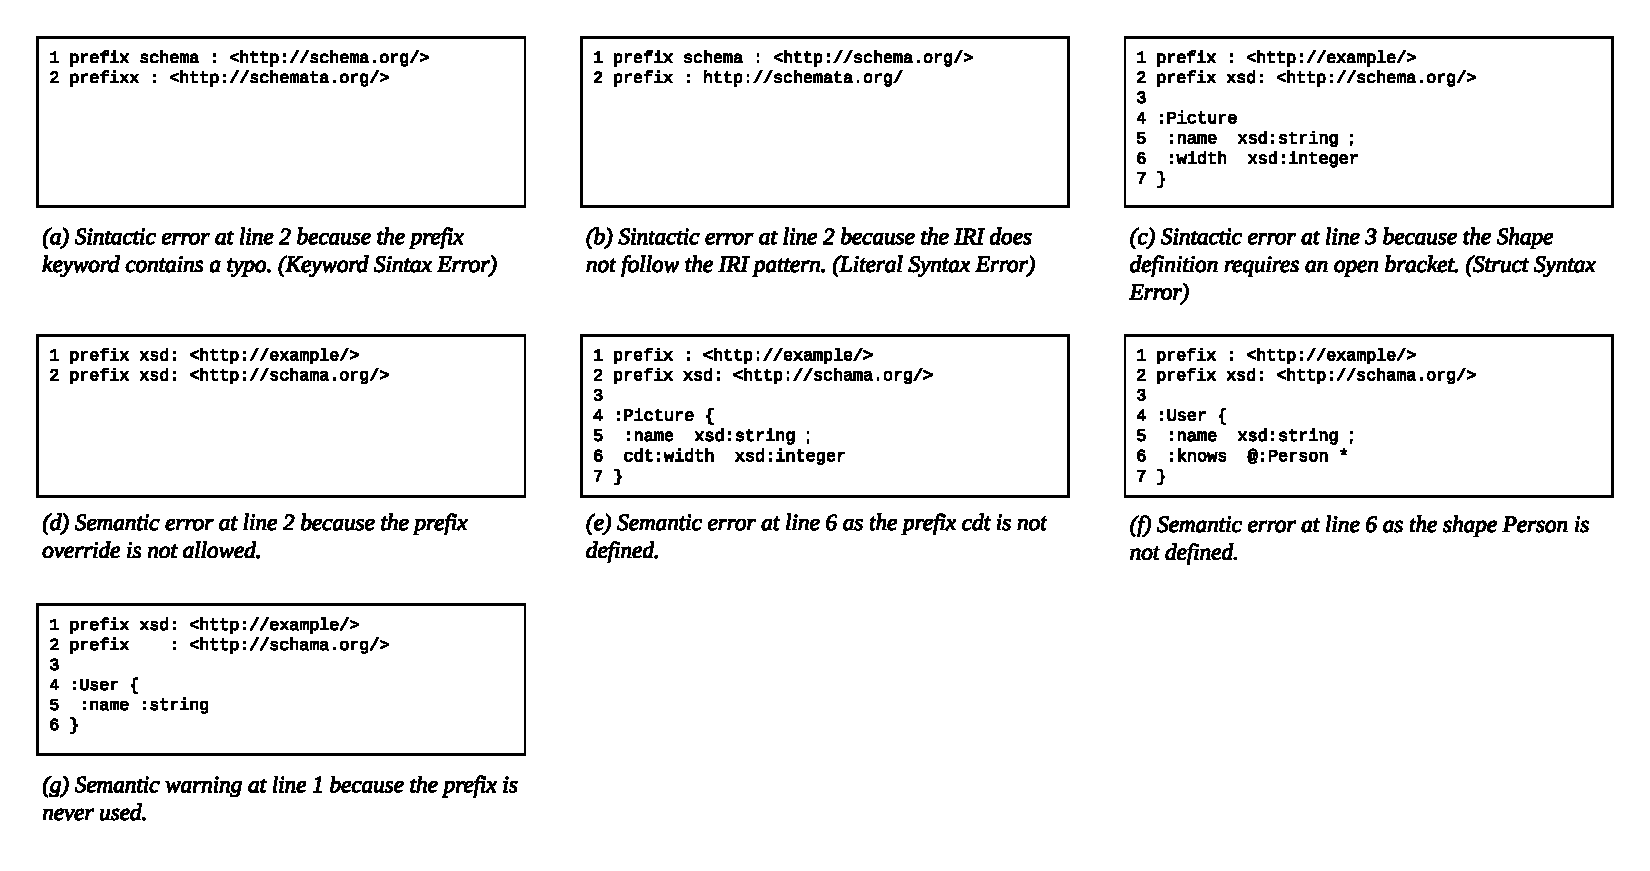
\includegraphics[width=\textwidth]{images/shexc-micro-bad-examples.pdf}
    \centering
    \caption[Examples of ShEx micro Compact Syntax code containing sintactic and semantic errors or warnings]{Examples of ShEx micro Compact Syntax
    code containing errors.}
    \label{fig:shexc-micro-errors}
  \end{figure}

\section{Sintactic Analyzers}
According to \cite{floyd1963syntactic} we consider a Sintactic Analyzer a piece of software capable of parse, generate
a parse tree and detect and emmit sintactic warnings and errors.

Therefore in this category we would include \textbf{Shaclex}, \textbf{ShEx.js}, \textbf{YASHE} and \textbf{VS Code Plugin}.
\cref{tb:sintactic-errors} shows a comparison between the analyzed tools.

Some comments to be made about the results obtained are that although we get an error for syntactic errors,
the quality of the error is more or less always the same. For example for the fragment \texttt{prefixx xsd: <http://example/>}
where we introduced an error at the keywork \texttt{prefix} by adding an extra \texttt{x} the error obtained is: \texttt{This line is invalid. Expected: PNAME\_NS.}

To our point of view this error message nor is not correct because it does not provide the user enough information to fix the schema.

Then also it is important to remark that during this analysis we encounter other sintactic problems that where not detected by tools like Shaclex,
an exmaple is that properties like \texttt{schema:rdf@:name} \textit{(which is not a valid IRI)} are accepted without errors.

\begin{table}
  \centering
  \caption{Detection of the different sintactic errors by the current existing ShEx tools that sintactically analyze the
  shape expressions.}
  \label{tb:sintactic-errors}
  \resizebox{\textwidth}{!}{\begin{tabular}{lcccccccc} 
    \hline\hline
                   & \multicolumn{8}{c}{Sintactic Errors}                                                                                                                                                                                                                                                                                                                          \\ 
    \hline
    Analyzers      & \multicolumn{1}{l}{Prefix Definition} & \multicolumn{1}{l}{Base Definition} & \multicolumn{1}{l}{Start Shape} & \multicolumn{1}{l}{Shape Definition} & \multicolumn{1}{l}{Prefix Reference} & \multicolumn{1}{l}{Base Reference} & \multicolumn{1}{l}{Shape Reference} & \begin{tabular}[c]{@{}c@{}}Recomends Semicolon\\Last Triple Constraint\end{tabular}  \\ 
    \hline
    Shaclex        & Yes                                   & Yes                                 & Yes                             & Yes                                  & Not completly                        & Yes                                & Yes                                 & No                                                                                   \\
    ShEx.js        & Yes                                   & Yes                                 & Yes                             & Yes                                  & Yes                                  & Yes                                & Yes                                 & No                                                                                   \\
    YASHE          & Yes                                   & Yes                                 & Yes                             & Yes                                  & Yes                                  & Yes                                & Yes                                 & No                                                                                   \\
    VS Code Plugin & Yes                                   & Yes                                 & Yes                             & Yes                                  & Yes                                  & Yes                                & Yes                                 & No                                                                                   \\
    \hline
    \end{tabular}}
\end{table}

\section{Semantic Analyzers}
As Semantic Analyzers we will only consider those tools that validate the semantics of the language, in this section we
include the validation of references like prefixes and shapes. The tools that claim to support this validations are
\textbf{Shaclex}, \textbf{ShEx.js}, and \textbf{YASHE}. \cref{tb:semantic-errors} shows a comparison between the analyzed tools.

From the obtained results we have to point that most of the tools opted for an open policy when talking about language semantics. From our
point of view this have its advantages and its drawbaks. But this only affects to the override policy. All of the tools should
implement the non existing references validation and most of them only focus on prefixes definition with the exception of
YASHE which does the checking of the shape reference but the error message sometimes is not completly accurate.

It it also remarkable that none of the tools performs a deeper analysis so there is no detection of unused resources, therefore
no warnings are generated by none of the existing tools.

\begin{table}
  \centering
  \caption{Detection of the different semantic errors by the current existing ShEx tools that semantically analyze the
  shape expressions.}
  \label{tb:semantic-errors}
  \resizebox{\textwidth}{!}{\begin{tabular}{lccccccc} 
    \hline\hline
                   & \multicolumn{7}{c}{Semantic Errors}                                                                                                                                                                                                                                                                                                                                                 \\ 
    \hline
    Analyzers      & \multicolumn{1}{l}{Prefix Override} & \multicolumn{1}{l}{Base Override} & \multicolumn{1}{l}{Start Shape Override} & \multicolumn{1}{l}{Shape Override} & \begin{tabular}[c]{@{}c@{}}Non Existing\\Prefix Reference \end{tabular} & \begin{tabular}[c]{@{}c@{}}Non Existing\\Base Reference \end{tabular} & \begin{tabular}[c]{@{}c@{}}Non Existing\\Shape Reference \end{tabular}  \\ 
    \hline
    Shaclex        & No                                  & No                                & No                                       & No                                 & Yes                                                                     & -                                                                     & No                                                                      \\
    ShEx.js        & No                                  & No                                & No                                       & No                                 & Yes                                                                     & -                                                                     & No                                                                      \\
    YASHE          & No                                  & No                                & No                                       & No                                 & Yes                                                                     & -                                                                     & Yes\footnote{When in the shape reference the prefix is the reference that is not right it still indicates that the shape is the one not existing.}                                                                     \\
    \hline
    \end{tabular}}
\end{table}

\section{Possible Enhancements}
Previous sections show the current state of the existing tools, their capabilities and their lacks.
With all that information we propose a list of enhancements that can be done to improve the error and warning detection
As seen in previus sections there's work that can be done to improve the existing ecosystem of tools. We have identified the following aspects
that will benefit end users:

\begin{itemize}
    \item \textbf{Enhancement of error messages.} Existing error messages, originated both by sintactic or semantic errors do not offer information about
    the exact place that originates the error nor a processed description nor possible solutions.
    \item \textbf{Creation of a new type of error messages with lower importance called warnings.} Currently systems do not analyze if declared resources are
    used and therefore there is no need to generate warnings. We propose to not only fully analyze the resources to detect non-used ones but also the creation
    or error messages with lower importance like warnings that can be used to offer more information to the end user.
    \item \textbf{Detection of override definitions.} Most of the existing tools prefer not to detect when a definition is being overriden, we propose to detect those
    situations and treat definitions as fixed values.
    \item \textbf{Detection of undefined references.} Some tools detect some broken references, we propose to enchace this situation and take that behaviour to
    other elements like shape references.
    \item \textbf{Detection of unused resources.} Related to the second point sometimes new users copy and paste old code which ends with lots of unused code,
    we propose a system that detects those situations and suggest to remove that unused code.
\end{itemize}
	\chapter{Proposed Sintactic and Semantic Analyzer}
\label{ch:proposed-sintactic-semantic-analyzer}

Once all the objectives and requirements to be achieved have been described,
the different systems and techniques existing to achieve them have been studied,
and their contributions and shortcomings have been evaluated, we will describe
the proposed solution both in terms of design and possible implementation

\section{Structure}
The system is divided into components so that each component works on its input
and produces its output. In this way, a parser is achieved that behaves like
an API where each element can be called individually. \cref{fig:shex-lite-sema}
shows the different components of this analyzer.

\begin{figure}
    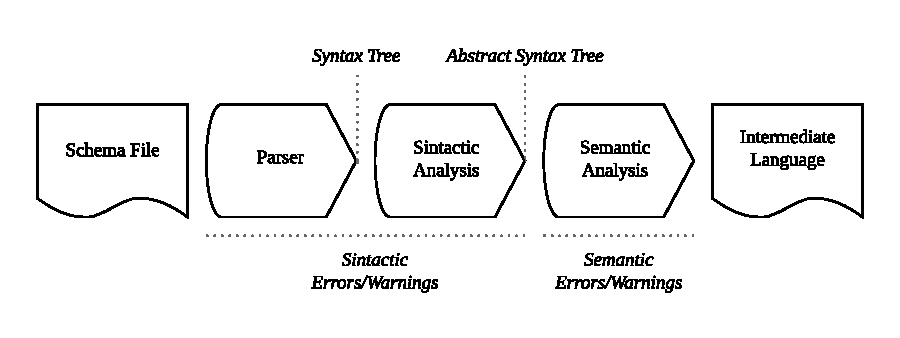
\includegraphics[width=\textwidth]{images/sin-sem-structure.pdf}
    \centering
    \caption[Sintactic and Semantic Analyzer structure]{Sintactic and Semantic Analyzer structure.}
    \label{fig:shex-lite-sema}
\end{figure}

\subsection{Parser}
We define the parsing stage as the process that begins when we receive the source code that makes up
the schema until the moment we produce a syntax tree. Therefore it includes the conversion to tokens
by the lexer, the grouping of tokens in rules and later in a syntax tree by the parser.

The general idea of this stage is that you take the source code as input and build a syntactic tree with all
the possible information from the source code. This implies that the syntactic tree is not only made up of
abstract grammar, but also of separators, braces and keywords. \cref{fig:shex-lite-st} shows an example
of the first 20 nodes generated by the parser. There we can see this composition of separators, keywords, braces
and content.

\begin{figure}
    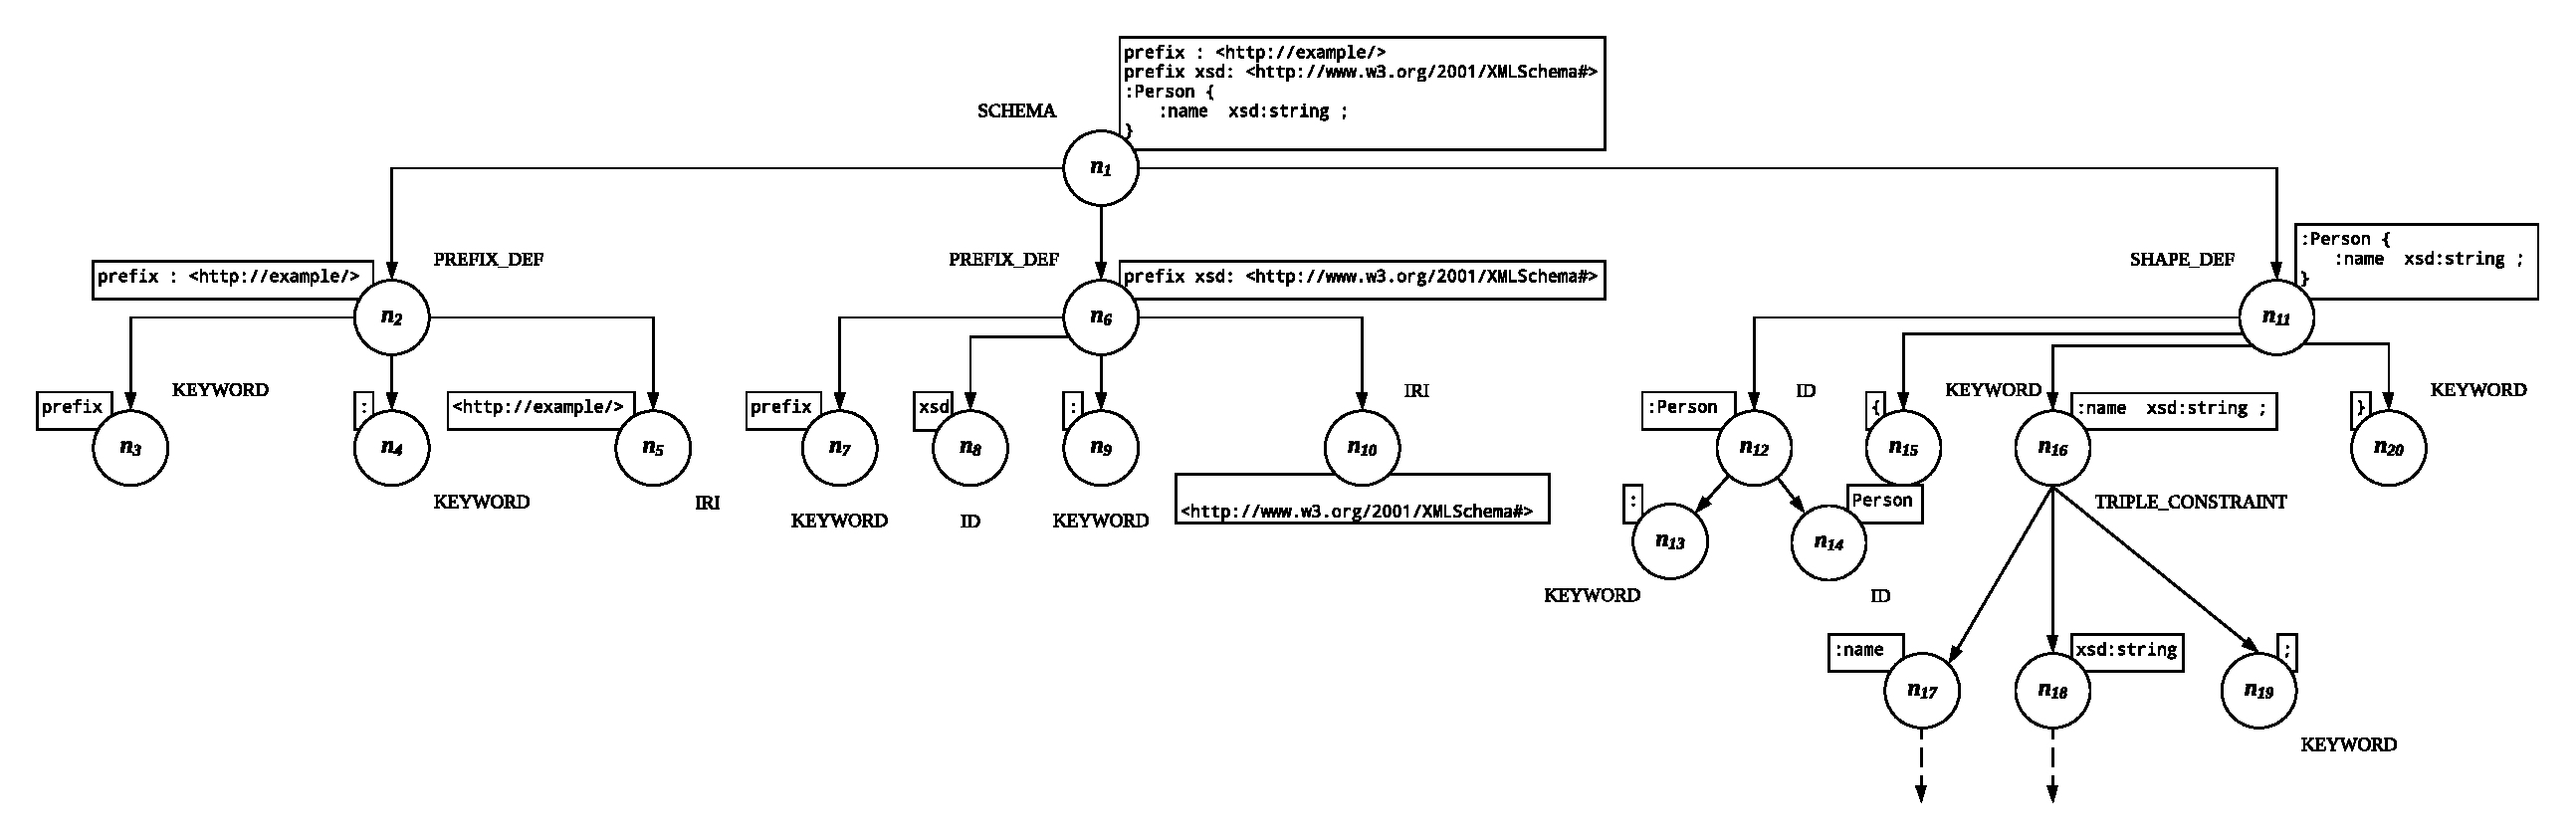
\includegraphics[width=\textwidth]{images/shex-lite-syntax-tree.pdf}
    \centering
    \caption[Syntax Tree tweenty first nodes produced by the parser]{Syntax Tree tweenty first nodes produced by the parser.}
    \label{fig:shex-lite-st}
\end{figure}

Once we have the complete syntactic tree generated, we can go through it to carry out syntactic analysis on the different elements.
For example, in the tree in \cref{fig:shex-lite-st} we could implement a validator that in the event that the last triple constraint
of a shape definition \textit{(node 16)} did not have the semicolon termination keyword \textit{(node 19)}, it would generate a
warning message to the user.

\subsection{Sintactic Analyzer}
The sintactic analyzer is in charge of traversing the syntactic tree in order to search for possible patterns that the user has to
be informed about. If none were found it would be understood that the syntactic tree is well formed and it will tranform the Syntax Tree
\cref{fig:shex-lite-st} into an Abstract Syntax Tree \cref{fig:shex-lite-sema-anal} \textit{(without the green and red relations)}.

For this, each node within our syntactic tree is aware of the context in which it is. Therefore we can ask questions to the nodes,
such as to a prefix definition \textit{(\cref{fig:shex-lite-st} $n_2$)}, do you have a label? \textit{(No)} or who is the node
that defines your iri? \textit{(node $n_5$)}. With questions like these, the syntactic tree can be analyzed for patterns that
represent warnings or errors.

\subsection{Semantic Analyzer}
The semantic analyzer is responsible of building all the possible relations between the AST nodes, analyze and check that
all those relations that must exist indeed exist. For this porpouse as just seen we reduce our Syntax Tree to an
Abstract Syntax Tree. \cref{fig:shex-lite-sema-anal} Shows a the resulting AST after the correspinding analysis and
transformations, we call this graph the \textit{Intermediate Language}.

\begin{figure}
    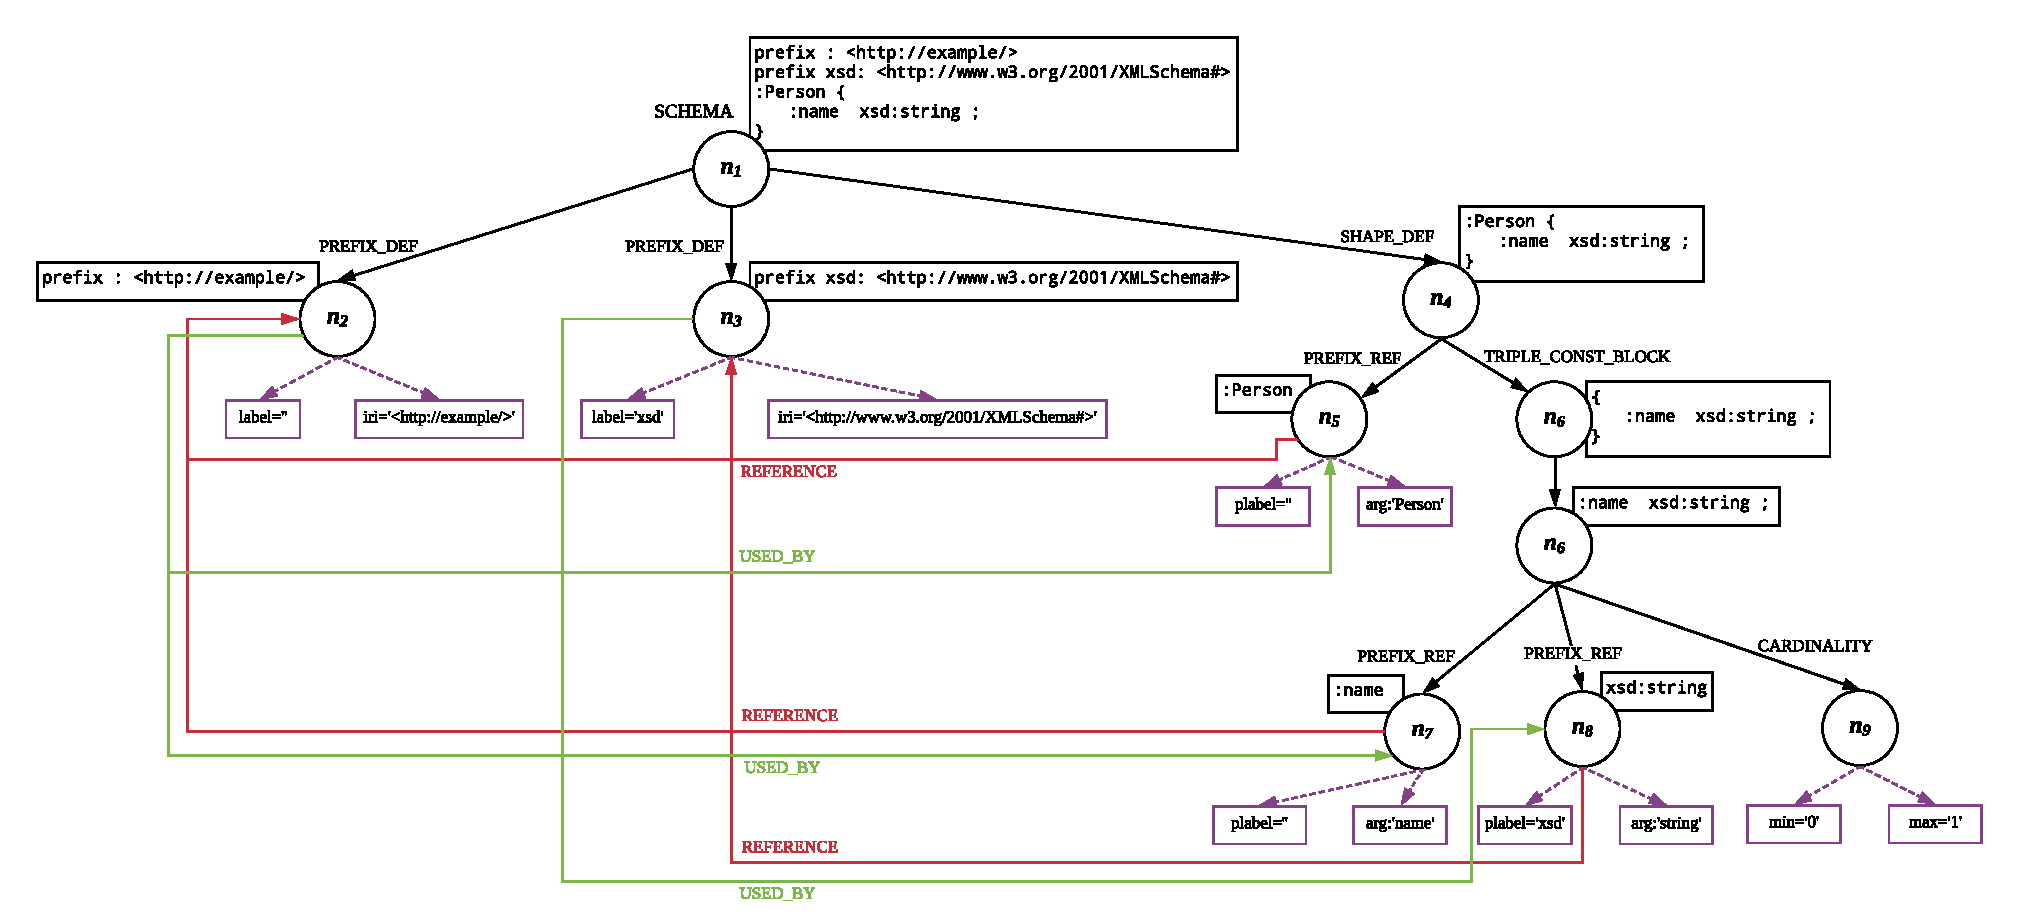
\includegraphics[width=\textwidth]{images/shex-lite-sema-anal.pdf}
    \centering
    \caption[Abstract Syntax Tree produced after validation and transformations]{Abstract Syntax Tree produced after validation and
    transformations.}
    \label{fig:shex-lite-sema-anal}
\end{figure}

Once we have the representation modeled and this representation is capable of expressing all the assumptions of our language,
we can begin to apply validators on our structure. For example if we wanted to find broken references we could go to the nodes
that are a reference to definitions like nodes $n_{\:5,\:7\:and\:8}$ and check that there is indeed a valid reference for each of them.

Furthermore, we can even analyze how many times a definition is used by a reference so that we can launch messages warning the end user
in some cases, such as when a prefix is not used.

\section{Implementation}\label{sec:anal-implementation}
As proof of concept of the previous proposal we offer an implementation of the three components, the parser, the sintactic analyzer
and the semantic parser. The implementation is defined in the same way as the structure, in three parts. We will now explore each
of those parts and their responsibilities separately.

\subsection{Parser}
As previously discussed, the function of the parser is to extract a syntactic tree from the diagrams that we can analyze.
For this purpose we decided to use the Antlr tool \cite{parr1995antlr}. This tool is capable of generating sintactic analyzers
from grammars defined in its own syntax. However, this tool is focused on completely processing the syntax tree and producing
only the abstract syntax tree. Therefore we had to use a modification of the original ShEx micro Compact Syntax syntax so that
Antlr would produce a tree with all the syntactic content. This also does offer the flexibility that in the future if we want to
implement any additional syntactic validation we simply have to do it on the tree that the parser generates for
us and not on the Antlr code.

\subsection{Sintactic Analizer}
The sintactic analyzer has the responsibility to validate that the parser produced syntax tree is correct and to build the abstract syntax
tree as well. To do this, it uses the same mechanism. Through the visitor pattern we go through our syntax tree. Each implementation
of this visitor has a purpose, for example an implementation can go through a few specific nodes to validate them syntactically
while another can go through them in order to build the AST. \cref{fig:checker-example} shows an example of how a sintactic check is
implemented.

\begin{figure}
    \begin{lstlisting}[language=Java,numbers=left,basicstyle=\ttfamily\scriptsize]
override def visitConstraint_triple_expr(...) {
  if(/*No trailing semicolon*/)
    //Warn user about this bad practice
}
    \end{lstlisting}
    \caption[Checker implementation for missing semicolons warning generation]{Checker implementation for missing semicolons warning generation.}
    \label{fig:checker-example}
\end{figure}

The AST construction stage is very delicate since for each generated node we have to include as much context information as possible
so that when an error is detected in the tree we can identify not only the cause but also the position, the origin, the rest of the
affected nodes and therefore offer a content-rich error message. Regarding our implementation, for each node we save the following
context information:
\begin{itemize}
    \item \textbf{Source file path.} Represents the path to the source file where the node was generated.
    \item \textbf{Line.} The line in the source file where the node was generated.
    \item \textbf{Column.} The column in the source file where the node was generated.
    \item \textbf{Token interval.} The interval \textit{(start, end position)} of tokens from the source file that generated the node.
    \item \textbf{Content.} The content of the node as plain text. \cref{fig:shex-lite-sema-anal} is very representative of this. 
    \item \textbf{Parent node.} A pointer to the parent node.
    \item \textbf{Children nodes.} A list of pointers to all the children nodes.
\end{itemize}

\cref{fig:shex-lite-node-info} represents this information inside each node. Our default implementation only looks for the
following extra syntactic pattern to the other implementations seen in \cref{ch:current-analyzers-analysis}: shape expressions whose last
triple constraint does not contain the semicolon ending character. In case we find this pattern, we inform the event manager
that a notice has been found that must be passed on to the user, \cref{fig:sin-err-example}.

\begin{figure}
    \begin{lstlisting}[numbers=left,basicstyle=\ttfamily\scriptsize]
warning[W005]: missing semicolon
--> shape_with_warning_cause_semicolon.shexl:8:23
    |
8   | :knows      @:User *
    |                      ^ semicolons are not compulsory in the last triple constraint,
                             but its usage its encouraged as otherwise your code wont be
                             following shape expressions specification.
    \end{lstlisting}
    \caption[Sintactic warning produced by the proposed sintactic analyzer]{Sintactic warning produced by the proposed sintactic analyzer.}
    \label{fig:sin-err-example}
\end{figure}

\begin{figure}
    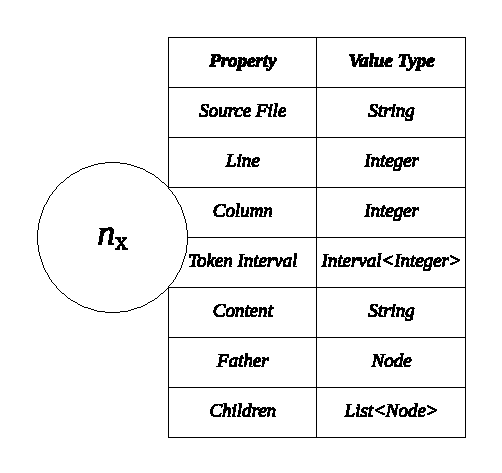
\includegraphics[scale=0.7]{images/shex-lite-node-table.pdf}
    \centering
    \caption[Common information stored at any AST node]{Common information stored at any AST node.}
    \label{fig:shex-lite-node-info}
\end{figure}

\subsection{Semantic Analizer}
Recall that the semantic analyzer takes the generated AST, runs it in search of errors and transforms it in such a way that
it emits a graph that corresponds to the intermediate language. We can separate semantic analysis into two phases, a first
one in which we transform our syntactic tree, adding possible relationships. And a second phase in which we analyze existing
and created relationships.

\subsubsection{Tree transformations}
In the case of our syntax the semantic relations that we find is the linking of a reference to its definition and the opposite
direction to indicate that a definition is being referenced by a node. The transformations are listed bellow:

\begin{itemize}
    \item \textbf{Linking prefix definition with prefix references.} Prefix references occurs when a node describes itself as
    the composition of a prefix and an argument. The idea is that the prefix subtitute the IRI, but must be linked as any
    prefix reference needs to point to an existing definition.
    \item \textbf{Linking base definition with base references.} Some nodes are defined as relative IRIs to the base definition
    and therefore need to be linking to them in order to be able to get that base IRI.
    \item \textbf{Linking shape definition with a shape reference.} Shape definitions can be used at the \texttt{start} definition
    to point the deafult shape or as type constraints in the triple constraints. At any of those points shape references must
    exist within the scope of an schema.
\end{itemize}

\subsubsection{Tree relations analysis}
For this purpose, the semantic analizer defines the visitor pattern on the nodes of the abstract syntax tree so that each of the different
analysis is done with a tree visiting implementation. Some of the 

\section{Sintactic and Semantic Error and Warnings Detected}
With the solution proposed in the previous section, our system is capable of detecting and reporting multiple syntactic
and / or semantic errors. In this section we will analyze the rules that generate each type of event and the different
error messages produced for each of them.

\subsection{Not trailing semicolon at last triple constraint}
To detect when the semicolon is missing in the last triple constraint of a shape definition, the rule used is very simple.
Find the last node in the triple constraints list of a shape definition. And once this node is found, it is searched whether or
not it contains the final token character that corresponds to a semicolon. If it does not have it, a warning message is generated,
indicating the position through file, line, column and context, which is sent to the compilation event manager, which in turn gives
the corresponding format to print the message. \cref{fig:sin-err-example} shows an example of this message.

\subsection{Prefix not defined}
These types of events happen when we use a referecnai to a prefix and this has not been defined in the scope of the schema.
In the event that this happens we have an error that we cannot recover from since we cannot associate the reference to anything.

In order to detect this assumption, all the prefix definitions have to be traversed previously and for each one of them,
a record will have to be created in a symbol table where it is indexed by the label and a reference to the definition node
is added. All types of type reference to prefix can then be accessed and for each one it is verified that the label exists
in the symbol table and then a pointer to the corresponding definition node is added to the reference node. If, on the other hand,
a definition cannot be found in the symbol table, then an error message like \cref{fig:err-non-def-pref} is created.

For example in the \cref{fig:shex-lite-sema-anal} the red lines would be the transformations done to the original AST to
add the pointers to the referece nodes that point to the definition nodes.

\begin{figure}
    \begin{lstlisting}[numbers=left,basicstyle=\ttfamily\scriptsize]
error[E007]: prefix not defined
--> shape_with_error_cause_pref_not_defined.shex:17:3
    |
17  | non_existing:label  xsd:string  +;
    | ^ the prefix `non_existing` has not been defined
    \end{lstlisting}
    \caption[Semantic error produced by an undefined prefix]{Semantic error produced by an undefined prefix.}
    \label{fig:err-non-def-pref}
\end{figure}

\subsection{Shape not defined}
In the same way as the previous case, an undefined shape error occurs in the case that there is a reference to a shape
expression that is not defined in the scope of the schema.

For this, all the definitions of shape expressions of our schema must have been previously identified and indexed in
a symbol table where the key is the name and the value a reference to the node of the definition. Once the definitions
of shape expressions have been identified, we only have to go through those nodes of type reference to shape expression
and look for a definition of a shape expression with the corresponding label within the scope of the prefix specified
in the reference. If it exists, a reference is added to the type reference to shape that points to the corresponding
definition. Otherwise, an error message like \cref{fig:err-non-def-shape} is generated.

\begin{figure}
    \begin{lstlisting}[numbers=left,basicstyle=\ttfamily\scriptsize]
error[E008]: shape not defined
--> shape_with_error_cause_shape_not_defined.shex:16:13
    |
16  | @existing_prefix:Not_Existing_Shape
    |                  ^ the shape `Not_Existing_Shape` has not been defined
                         in the scope of the prefix `existing_prefix`
    \end{lstlisting}
    \caption[Semantic error produced by an undefined shape]{Semantic error produced by an undefined shape.}
    \label{fig:err-non-def-shape}
\end{figure}

\subsection{Prefix overriden}
We say that a prefix is overwritten when we come across a second prefix definition that tries to assign any
value to a prefix that had already been defined previously.

For this, during the identification of prefixes, every time we find a prefix type node we try to add a record
to our symbol table. In this entry, the key will be the prefix label. If there is already an entry in the symbol
table with the same tag, then we would be facing a prefix override. So instead of taking the action we would
throw an error message like \cref{fig:err-override-prefix}.

\begin{figure}
    \begin{lstlisting}[numbers=left,basicstyle=\ttfamily\scriptsize]
error[E003]: attempt to override an already defined prefix
--> shape_with_error_cause_prefix_override.shex:15:0
    |
15  | PREFIX foaf: <hppt://another/value>
    | ^ this prefix definition overrides the previous one (9:0) with
        value <http://xmlns.com/foaf/0.1/>
    \end{lstlisting}
    \caption[Semantic error produced by a prefix override]{Semantic error produced by a prefix override.}
    \label{fig:err-override-prefix}
\end{figure}

\subsection{Shape overriden}
The case of a shape expression overwriting is slightly less trivial in that a shape is identified as the
union of an existing prefix and a unique identifier within the ambit of that prefix. Therefore, the way
of acting will be (assuming that the prefix exists, if it would not be another error) check if a shape
definition with the same identifier already exists within the scope of the indicated prefix. If it exists
we will throw an error like the one from \cref{fig:err-override-shape}. If not, we will add a record to the
indicated prefix scope with the corresponding information from the shape definition.

\begin{figure}
    \begin{lstlisting}[numbers=left,basicstyle=\ttfamily\scriptsize]
error[E004]: attempt to override an already defined shape
--> shape_with_error_cause_shape_override.shex:40:0
    |
40  | :Q3559 {
    |  ^ this shape definition overrides the previous one (17:0)
41  |   schema:name xsd:string ;
42  | }
    \end{lstlisting}
    \caption[Semantic error produced by a shape override]{Semantic error produced by a shape override.}
    \label{fig:err-override-shape}
\end{figure}

\subsection{Unused prefix definition}
One of the small optimizations that our semantic solution includes is the early detection of resources
not defined as prefixes. In addition, it is a use case of semantic statistics generated by our proposed
solution. In this specific case, what is checked is the number of resources that use a definition. For this,
the symbol table is consulted since this is the one that stores this information. It corresponds to the
relationships in green in \cref{fig:shex-lite-sema-anal}.

In the event that a prefix definition has zero resources that use it, the prefix is not used and therefore
it can be removed without problem since it only takes up space. To warn the user of this, a warning like \cref{fig:warn-pref-not-used}
is generated

\begin{figure}
    \begin{lstlisting}[numbers=left,basicstyle=\ttfamily\scriptsize]
warning[W001]: prefix definition not used
--> shape_with_warning_cause_prefix_never_used.shex:8:12
    |
8   | PREFIX owl: <http://www.w3.org/2002/07/owl#>
    |        ^ the prefix `owl` definition is never used
    \end{lstlisting}
    \caption[Semantic warning produced by a prefix never used]{Semantic warning produced by a prefix never used.}
    \label{fig:warn-pref-not-used}
\end{figure}

\subsection{Base set but not used}
Another case in which the early detection of unused resources is used is with the definition of the base.
If for some reason a user assigns a value to the base but never uses it, a warning like \cref{fig:warn-base-not-used}
is generated.

\begin{figure}
\begin{lstlisting}[numbers=left,basicstyle=\ttfamily\scriptsize]
warning[W002]: base has been set but not used
--> shape_with_warning_cause_base_set_but_never_used.shex:17:5
    |
17  | BASE <http://a/base/not/used/value>
    |      ^ the base `<http://a/base/not/used/value>` definition is
             set but not used
    \end{lstlisting}
    \caption[Semantic warning produced by a base set but never used]{Semantic warning produced by a base set but never used.}
    \label{fig:warn-base-not-used}
\end{figure}

	\part{Translating ShEx Schemas to Object Domain Models}
	\chapter{Object Domain Model Translation Problem}
\label{ch:odm-transl}

The ODMTP \textit{(Object Domain Model Translation Problem)}, when talking about
Shape Expressions, is the aim to transform existing schemas, that already represent
domain models, in to object domain models. Or what it is the same, translate the ShEx
schemas to objects coded in some Object Oriented Language. \cref{fig:shex-translate-small}
represents this aim. The problem is to convert the \textit{Source} in to the \textit{Target}
($shex \rightarrow object\ oriented\ language$).

\begin{center}
	\noindent\begin{minipage}[t]{.4\textwidth}
        \begin{lstlisting}[frame=topline,numbers=left,title=\scriptsize{Person Schema (Source)},
            basicstyle=\ttfamily\scriptsize]{a}
# Prefixes...
:Person {
	:name xsd:string ;
	:knows @:Person *
}
		\end{lstlisting}
	\end{minipage}\hfill
	\begin{minipage}[t]{.5\textwidth}
        \begin{lstlisting}[language=Java, frame=t,numbers=left,title=\scriptsize{Person Java Object (Target)},
            basicstyle=\ttfamily\scriptsize]{b}
// Imports...
public class Person {
	private String name;
	private List<Person> knows;
	// Constructor...
	// Getters and Setters...
}
		\end{lstlisting}
	\end{minipage}
    \captionof{figure}{Schema modeling a \texttt{Person} in \texttt{ShExC} syntax to the left.
    And the expected translated code in \texttt{Java} to the right.}
	\label{fig:shex-translate-small}
\end{center}

This problem, with the previous example \cref{fig:shex-translate-small}, may seem simple to solve, however,
before proposing a solution, we need to explore if everything that can be expressed with ShEx can be
expressed in object-oriented languages.

To answer this question, we will reduce our problem by using the micro ShEx syntax and PO \textit{(Plain Objects)}
\cite{fowler1997analysis} as a generalization of all the programming languages that support the object orientated
paradigm. Therefore our study will focus on finding out if we can express in plain objects everything we can express
in the ShEx micro syntax. \cref{eq:expressivity-question} illustrates this question where $e(x)$ measures the
expressivity \cite{felleisen1991expressive} of $x$.

\begin{equation} \label{eq:expressivity-question}
    e(shex\ micro\ syntax) \leq e(plain\ objects)
\end{equation}

So, the first step will be to measure the expressivities of both the ShEx micro syntax and the Plain Objects to later
compare them.

% S E C T I O N   S H A P E   E X P R E S S I O N S   E X P R E S I V I T Y

\section{Shape Expressions Expressivity}
To measure the expressiveness of the ShEx micro syntax we will explore its abstract grammar \cref{fig:shex-micro-abstract-grammar}.

\begin{figure}
\begin{lstlisting}[numbers=left,basicstyle=\ttfamily\small]
schema           ::= definition+
definition       ::= prefixDef | baseDef | startDef | shapeDef
prefixDef        ::= ID IRI
baseDef          ::= IRI
startDef         ::= SHAPE_REF
shapeDef         ::= IRI_REF tripleConstraint+
tripleConstraint ::= IRI_REF constraint CARDINALITY
constraint       ::= IRI_REF | SHAPE_REF | "IRI" | "BNODE" |
                     "NONLITERAL" | "LITERAL"
\end{lstlisting}
\caption[ShEx Micro Abstract Grammar]{ShEx Micro Abstract Grammar.}
\label{fig:shex-micro-abstract-grammar}
\end{figure}

From the grammar we can infer that a shape is defined as an identifier and a set of triple expressions where each
triple expression is in turn defined as the property, which is a reference to a prefix, the constraint and the
cardinality. This, therefore, allows us to express that an object can be defined by one or by multiple properties,
each with a specific type. In addition, each of these properties that define the model can be repeated $n$ times,
indicated by the cardinality. \cref{fig:prop-def-shape-diagram} shows an example of a shape expression coded on
its micro compact syntax that defines two properties for the object \texttt{:Preson}.

\begin{figure}
    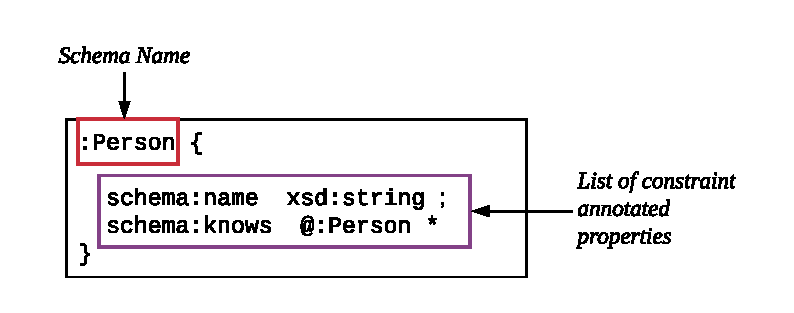
\includegraphics[scale=0.7]{images/shex-example-parts.pdf}
    \centering
    \caption[Shape expression modeling the properties of a Person]{Shape expression modeling the properties of a Person.}
    \label{fig:prop-def-shape-diagram}
\end{figure}

In that shape expression we can see that we have a property that represents the name with type string and the default cardinality \textit{(1)}.
And a second property \texttt{knows} whose type is a reference to another person and has multiple cardinality so it represents a list of people you know.

So we have just seen that a shape, in its reduced grammar is a set of triple expressions made up of the property, the type and the cardinality,
therefore we can formalize that a shape is defined as,

\begin{equation}\label{eq:shape-formalization}
shape_m \rightarrow \left \{ (p_{1m},t_{1m},c_{1m}),\ (p_{2m},t_{2m},c_{2m}),\ \dots,\ (p_{nm},t_{nm},c_{nm}) \right \}
\end{equation}

where $p_n \rightarrow property\ name\ of\ n$, $t_n \rightarrow type\ of\ n$ and $c_n \rightarrow cardinality\ of\ n$.
And therefore an schema is defined as,

\begin{equation}\label{eq:schema-formalization}
schema \rightarrow \left \{ shape_1,\ shape_2,\ \dots,\ shape_n \right \}
\end{equation}


% S E C T I O N   P L A I N   O B J E C T S   E X P R E S I V I T Y

\section{Plain Objects Expressivity}
Plain objects can be coded in any object oriented programming language, or at least in
any language that supports this paradigm. First we will explore how plain objects are 
generally coded, then how the language increases or decreases the expressivity and
finally we will generalize the core concepts that can be expressed by any plain object
codification.

\begin{figure}
    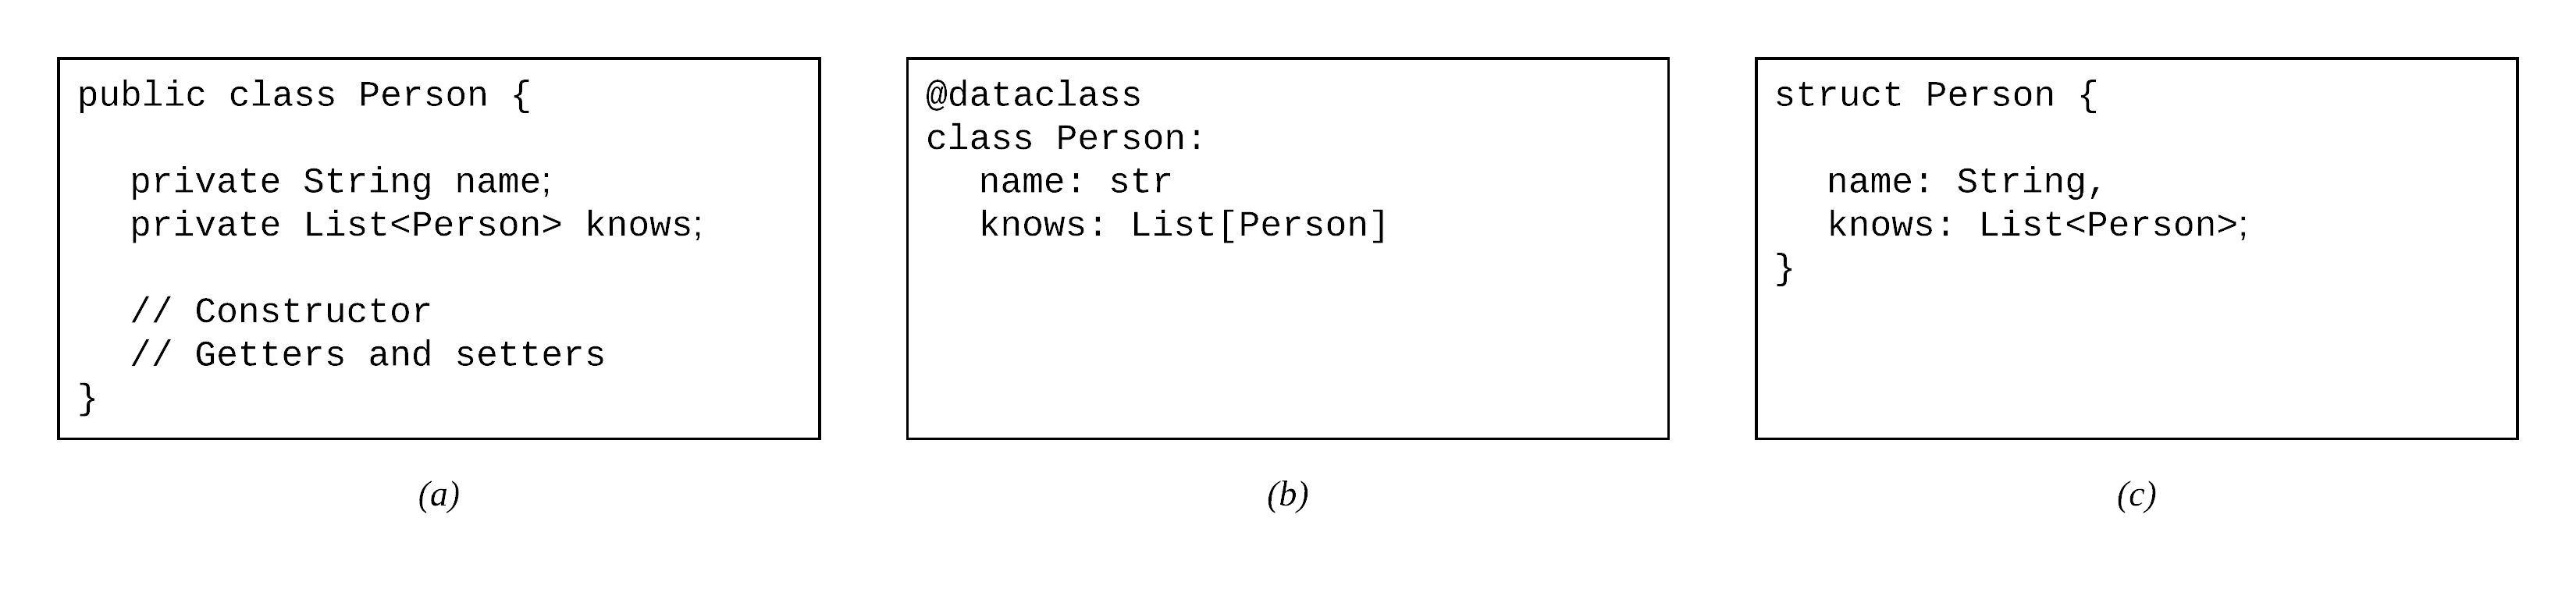
\includegraphics[width=\textwidth]{images/codings-exmaple.png}
    \centering
    \caption[Java, Python and Rust codings of Person object.]{Java, Python and Rust codings of Person object. 
    \textit{a} corresponds to Java, \textit{b} corresponds to Python and \textit{c} corresponds to Rust.}
    \label{fig:person-codings}
\end{figure}


\subsection{Plain Objects Structure}
From the existing programming languages we can infeer the general structure of plain objects. For this porpuse
we take the PYPL Index \textit{(PopularitY of Programming Language)} \footnote{\url{http://pypl.github.io/PYPL.html}}
from June 2020 and take the 2 most used programming languages that support the object oriented paradigm,
those would be Java and Python. And then, just to enlarge the scope we will take Rust because it is a new programming
language that includes lots of features.

\cref{fig:person-codings} shows three models that correspond to the codification of the Person schema from
\cref{fig:shex-translate-small}. For example if we analyze the Java fragment, that seems to be the most complex
one out of the three fragments we can see in \cref{fig:java-analysis} that it is composed by the \textit{Schema Name},
the \textit{List of Type Annotated Properties} and some \textit{Language Specific Code}. This corelates to the other
two programming languages as they also contain this three elements. Therefore after this brief analysis we can generalize that,

\begin{equation}\label{eq:plain-object}
    plain\ object_m \rightarrow \left \{ (p_{1m}, t_{1m}),\ (p_{2m}, t_{2m}),\ \dots,\ (p_{nm}, t_{nm}) \right \} + lsc
\end{equation}

where $p_n \rightarrow property\ name\ of\ n$, $t_n \rightarrow type\ of\ n$ and $lsc \rightarrow language\ specific\ code$.
And therefore a model based on plain objects is defined as,

\begin{equation}\label{eq:plain-object-model}
model \rightarrow \{ po_1,\ po_2,\ \dots,\ po_n \}
\end{equation}

where $po_n$ represents the plain object.

It is important to note that part of that language-specific code is responsible for representing the language-specific type system.
Therefore, before formalizing our generalization, we must explore whether the type system of a language affects its expressiveness
and, if so, find those types that are common to most languages of this type, if any.

\begin{figure}
    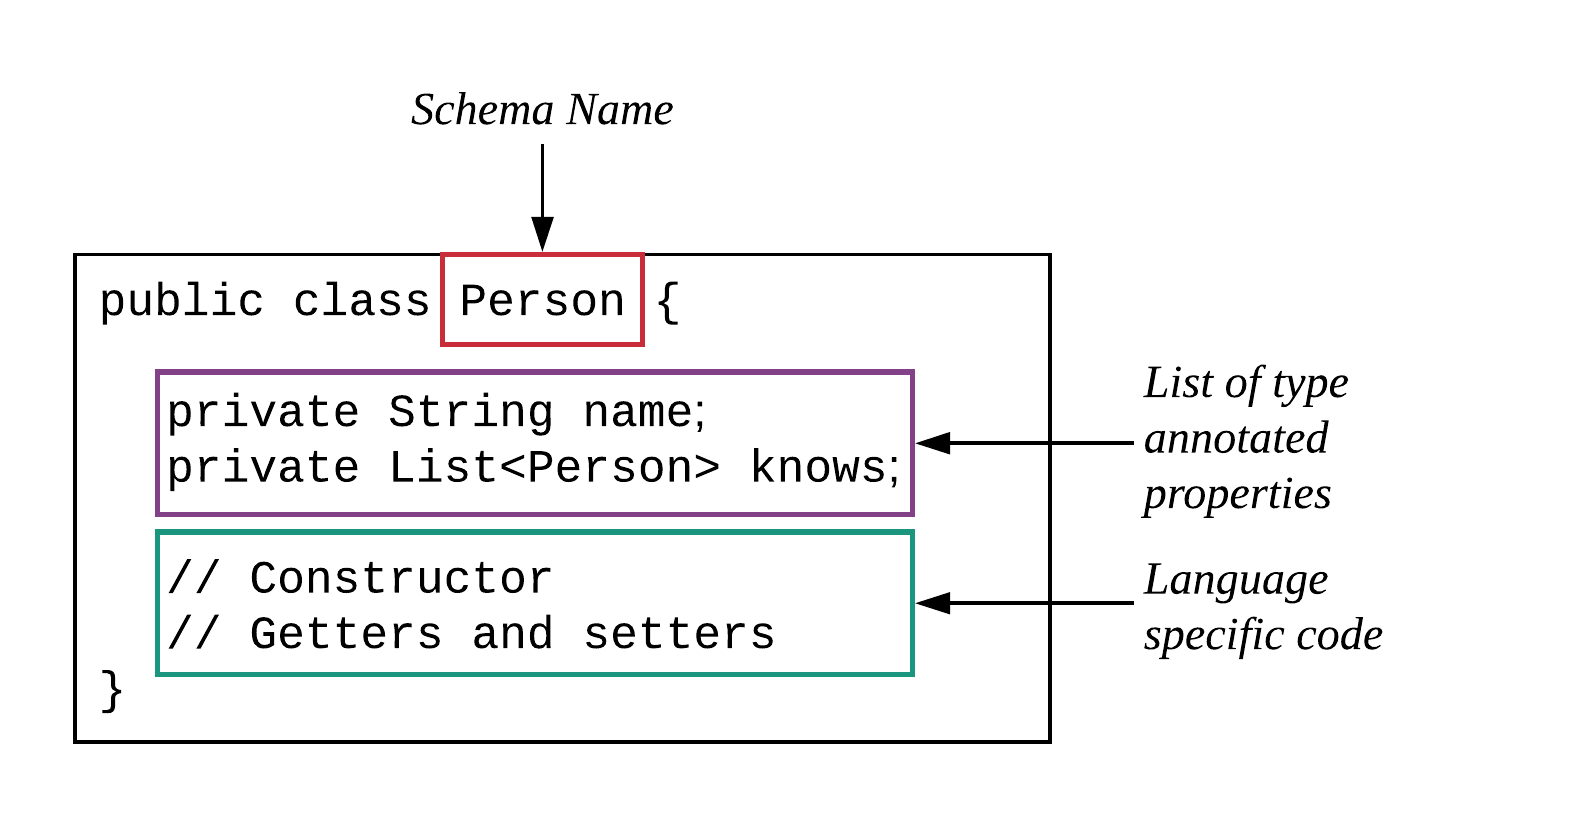
\includegraphics[scale=0.2]{images/java-analysis.png}
    \centering
    \caption[Java plain object decomposition.]{Java plain object decomposition.}
    \label{fig:java-analysis}
\end{figure}

\subsection{Plain Objects Language Expressivity Dependance}
In \cref{fig:person-codings} we can see that all of three languages use similar types to represent the Person model. But with
just one example we cannot generalize that the language does not affect the expressivity of the plain objects. In order to
test that condition and prove that the language affects or doesn't affect the expressivity of plain objects we will need first
to find two \textit{type-independent languages}.

\begin{definition}[Type-independent languages]
    Two languages $L_1$ and $L_2$ are type-independent if and only if one of the languages contains a type that cannot be
    represented by means of a linear combination of any other type of the other language.
\end{definition}

For example, lets take Java \textit{$L_1$} and Rust \textit{$L_2$}, examples \textit{(a)} and \textit{(c)} from \cref{fig:person-codings}.
Rust contains the type $Either<A,B>$, this type allows the type $A$ or $B$ and when accessed is not an $Either$ is either $A$ or $B$. In
Java there is no $Either$ type, and someone can say that we could achive a similar type by using inheritance and classes composition. But
at the end when accessed the type would be the type of the upper class. \textbf{Therefore Java and Rust are type-independent languages}.

Now in order to see if the expressivity depends on the types of a language let's assing values to Java and Rust by using the same
$Either<A,B>$ type. As can be see in \cref{fig:java-rust-comparison} Java does not allow to express the same as Rust is expressing
in this example. And therefore we can conclude that the expresivity of plain object is stronggly related to the build-in types that
the programming language in which they are coded provides.

\begin{center}
	\noindent\begin{minipage}[t]{.4\textwidth}
        \begin{lstlisting}[language=Java,frame=topline,numbers=left,title=\scriptsize{Person Rust Struct},
            basicstyle=\ttfamily\scriptsize]{a}
stuct Person {
    name: String,
    knows: List<Person>,
    owningPet: Either<Dog,Cat>,
}
		\end{lstlisting}
	\end{minipage}\hfill
	\begin{minipage}[t]{.5\textwidth}
        \begin{lstlisting}[language=Java, frame=t,numbers=left,title=\scriptsize{Person Java Object},
            basicstyle=\ttfamily\scriptsize]{b}
// Imports...
public class Person {
    private String name;
    private List<Person> knows;
    private Pet owningPet;
    // Constructor...
    // Getters and Setters...
}
		\end{lstlisting}
	\end{minipage}
    \captionof{figure}{Rust struct modeling a \texttt{Person} to the left.
    And the most similar approximation in Java to te right. In the Java approximation the Pet class is an interface
    that it is inherited by the Cat and Dog classes, that way we allow to store in the variable \texttt{owningPet}
    values of type Cat and Dog.}
	\label{fig:java-rust-comparison}
\end{center}


\subsection{Plain Objects Expressivity Generalization}
In order to obtain a generalization of the plain objects represented by means of object-oriented programming languages,
we will base ourselves on \cref{eq:plain-object} where we defined the composition of a flat object, in this way the
generalization would be as indicated in \cref{fig:po-generalization}. As can be seen this gneralization is not complete
as it does not include the production for the \texttt{type}. Thi is because we have not generalized the type system of the
object oriented programing languages yet.

\begin{figure}
    \begin{lstlisting}[numbers=left,basicstyle=\ttfamily\small]
    plain object     ::= (ID type)+
    \end{lstlisting}
    \caption[Plain Objects Partial Generalization]{Plain Objects Partial Generalization.}
    \label{fig:po-generalization}
\end{figure}

However and motivated not to over-extend the scope of this work instead of extracting a generalization for the possible types
that can be used in each object-oriented programming language, we will try to create this abstraction projecting it on the
most common types used by XML Schema (xsd) \cite{xmlschemasimpleelements}. The main reason is that in RDF, and therefore in ShEx, xsd is the most widely
used type system and the standard of w3c. This leads us to the generalization from \cref{fig:po-generalization-complete} where we re-use the
\texttt{xsd} types and add the \texttt{ID} that actually represents compound types, that is types that are in fact plain objects.

\begin{figure}
    \begin{lstlisting}[numbers=left,basicstyle=\ttfamily\small]
    plain object     ::= (ID type)+
    type             ::= INTEGER | DECIMAL | STRING | BOOLEAN | ID
    \end{lstlisting}
    \caption[Plain Objects Complete Generalization]{Plain Objects Complete Generalization.}
    \label{fig:po-generalization-complete}
\end{figure}

% S E C T I O N   C O M P A R I S O N 

\section{Shape Expressions and Plain Objects Expressivity Comparison}

Previous section cover the expressivity of Shape Expressions and Plain Objects, in this section we compare both expressivities and
expose if both expresivities are fully compatible or not. In \cref{eq:schema-formalization} we defined an schema and our aim to find if it is possible
to define a function $f$ such that $f(schema)\rightarrow model$ where $model$ is defined in \cref{eq:plain-object-model}. To achieve this function, it
is necessary that the expressiveness of the origin be less than or equal to that of the destination and now that we have already defined the
expressivities of each system we can compare them.

Let's simplify the problem by eliminating all those common factors that we have in both systems. For example, from \cref{eq:schema-formalization} and \cref{eq:plain-object-model}
we have lists of properties with something else, let's reduce the case to having a single property with something else like,
\begin{equation}
    (p_n,t_n,c_n);\ (p_n,t_n).
\end{equation}
Also in both cases we find that the property is a free text that identifies that property, so we eliminate it from the problem. And we are left with,
\begin{equation}
    (t_n,c_n);\ (t_n)
\end{equation}
where we need to find if the existis a function $f'$ such that we can map $(t_n,c_n)$ to $(t_n)$.

With the data that we currently have, we can now conclude that the expressiveness of the ShEx micro grammar is still greater than the
generalization proposed for plain objects, however this does not imply that there is no function $f$ that can map some schemas to
plain objects models. Furthermore, that means the opposite. From the current data we can ensure that there is at least a function $f$ capable of
mapping from shape expressions to plain object models provided that,

\begin{equation}\label{eq:constraint}
    t_n \in \left \{ string,\ integer,\ date,\ compoundObject \right \} and\ c_n \in \{ (1,1),\ (0,\infty)\}.
\end{equation}

That means that we will not be able to translate everything that can be expressed in ShEx Micro Compact Syntax but also means that we will be able
to at least translate some of the shapes. \cref{fig:mapping-f} illustrates this scenario. As you can see in the figure some shapes can be mapped, like the first two,
and other can't, like the third, in this case due to the cardinality not following the \cref{eq:constraint}.

\begin{figure}
    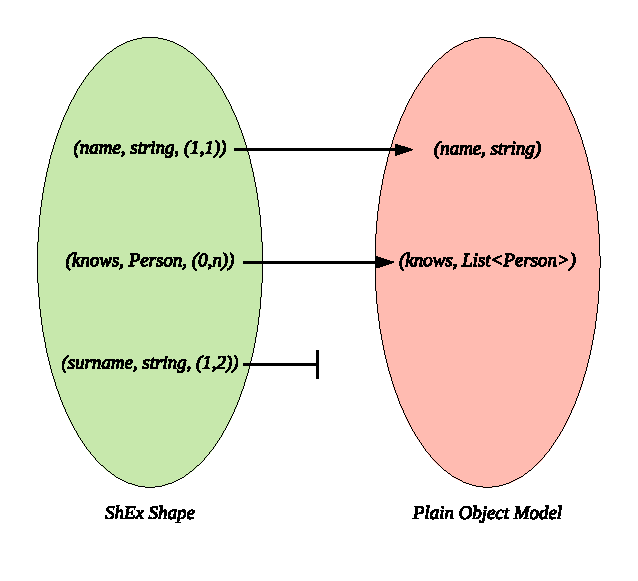
\includegraphics{images/shex-lite-mapping.pdf}
    \centering
    \caption[Mapping function from ShEx to Plain Object]{Mapping function from ShEx to Plain Object.}
    \label{fig:mapping-f}
\end{figure}
	\chapter{Proposed Translator}
\label{ch:proposed-system}

Para solucionar el problema expuesto en el punto 4, con toda esa información
proponemos una sintaxis basada en shexc que representa el subconjunto que podemos representar con PO.
Dicha sintaxis a demás al ser un subconjunto está validada semantica y sintácticamente de forma que
tiene más restricciones que shex normal, de forma que se aseguran las integridades del lenguage y
se propone un sistema de errores "actualizado". Para esta sintaxis ofrecemos tb un compilador
diseñado como una API que compila los esquemas que se realzian en esta sintaxis y los traduce al
lenguaje de programación objetivo que se desee.

\section{Structure}

\section{Generated Obejcts}

\begin{figure}
    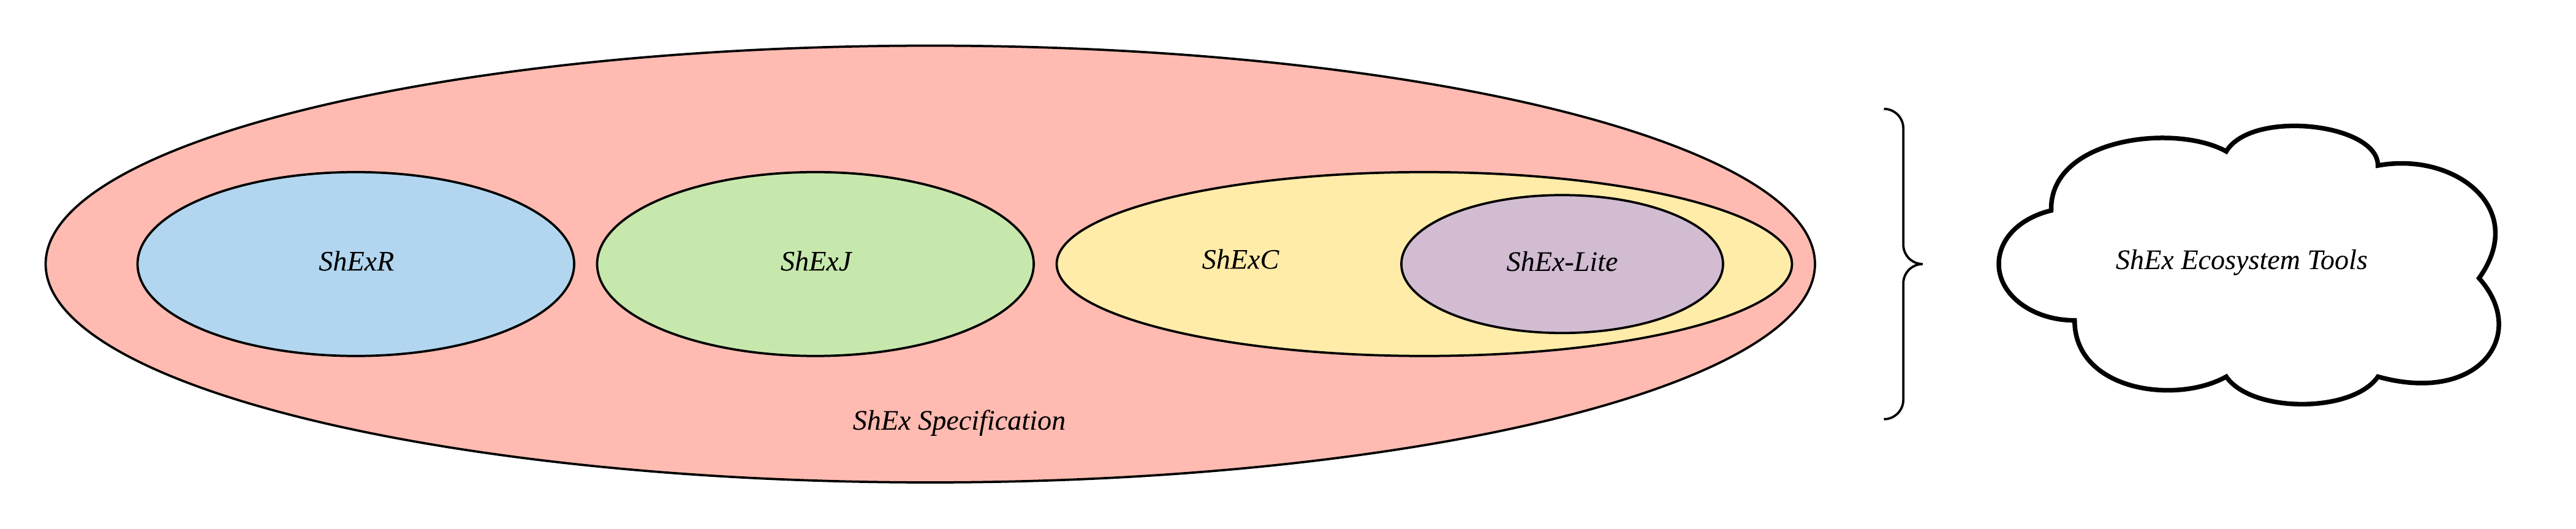
\includegraphics[width=\textwidth]{images/shex-lite-syntaxes-mental-model.png}
    \centering
    \caption[Mental model of ShEx-Lite in the existing ShEx syntaxes context.]{Mental model of
    ShEx-Lite in the existing ShEx syntaxes context. From this model we can see that Shex-Lite
    is in fact an strictly subset of ShExC, which follows the ShEx Specification. And therefore
    ShEx-Lite will also follow that expecification, which automatically enables ShEx-Lite schemas
    to be used in any other existing ShEx tool.}
    \label{fig:syntax-mental-model}
\end{figure}

\begin{figure}
  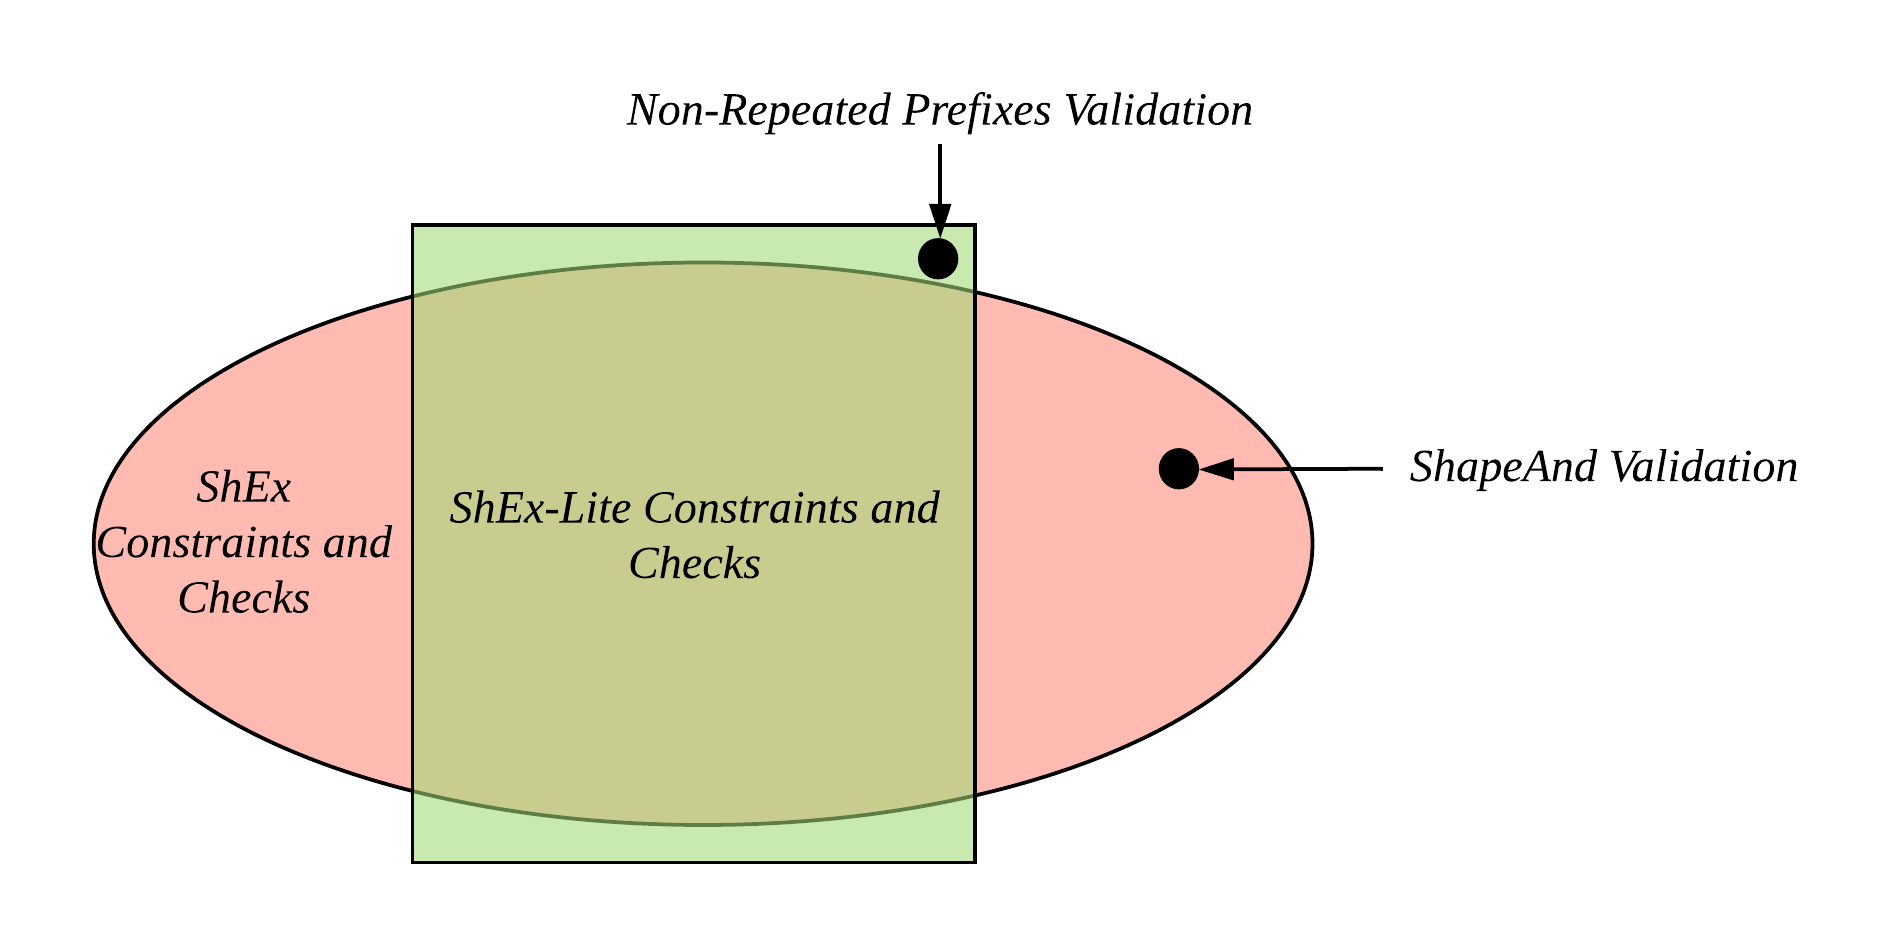
\includegraphics[width=\textwidth]{images/shex-lite-constraints-context.png}
  \centering
  \caption[Constraints and checks context diagram for ShEx-Lite and ShEx.]{Constraints
  and checks context diagram for ShEx-Lite and ShEx.}
  \label{fig:constraints-context}
\end{figure}

\begin{center}
	\noindent\begin{minipage}[t]{.4\textwidth}
		\begin{lstlisting}[frame=topline,numbers=left,title=\scriptsize\texttt{Person.shexl}, basicstyle=\ttfamily\scriptsize]{a}
# Prefixes...
:Person {
	:name xsd:string ;
	:knows @:Person *
}
		\end{lstlisting}
	\end{minipage}\hfill
	\begin{minipage}[t]{.5\textwidth}
		\begin{lstlisting}[language=Java, frame=t,numbers=left,title=\scriptsize\texttt{Person.java}, basicstyle=\ttfamily\scriptsize]{b}
// Imports...
public class Person {
	private String name;
	private List<Person> knows;
	// Constructor...
	// Getters and Setters...
}
		\end{lstlisting}
	\end{minipage}
	\captionof{figure}{Schema modeling a \texttt{Person} in \texttt{shexl} syntax to the left. And the \texttt{ShEx-Lite} generated code in \texttt{Java} to the right.}
	\label{fig:example-1}
\end{center}

	\part{Project Sinthesis}
	\chapter{Evaluation of Results}
\label{ch:results-evaluation}

\section{Methodology}
	\chapter{Planning and Budget}
\label{ch:planning-and-budget}

\section{Planning}
The planning of this work covers from the moment the proposal for the teaching commission began
to be made until the moment the work is presented publicly. Of course there are some milestones
that are fixed in time such as \textbf{the presentation of the proposal}, \textbf{the presentation of the dissertation}
and \textbf{the defense of the work}. Therefore planning revolves around these milestones \textit{(IDs
3, 4 and 5 from \cref{fig:planning-sheet})}.

\subsection{Presentation of the Proposal}
The acceptance of the proposal includes the first tasks \textit{(IDs
6-8 from \cref{fig:planning-sheet})} in which a small investigation is done on the
topics of interest and it is decided what the objectives to be pursued of the work will be.

In addition, it also includes the formal preparation of the proposal that will be delivered to the
management of the computer engineering school for evaluation.

\subsection{Presentation of the Dissertation}
To consider the presentation of the dissertation as complete, it is necessary to carry out the main
tasks \textit{(IDs 9-34 from \cref{fig:planning-sheet})} of the work, in our case they are to
carry out the corresponding research to understand the scope of the proposed objectives, to propose a
solution and to obtain a few relustados that can be empirically testable. So that we can evaluate our
solutions. And, of course, prepare the corresponding documentation that reflects all the work done.

\subsection{Defense of the Work}
The defense of the project corresponds to those tasks \textit{(IDs 34-36 from \cref{fig:planning-sheet})}
subsequent to the delivery of the dissertation and that have to do with public defense in which the work carried out is evaluated.

\bigskip
So as you can see the main project statistics are shown in \cref{tb:planning-stats}.

\begin{table}
    \caption[Statistics of the main project tasks]{Statistics of the main project tasks.}
    \label{tb:planning-stats}
    \centering
    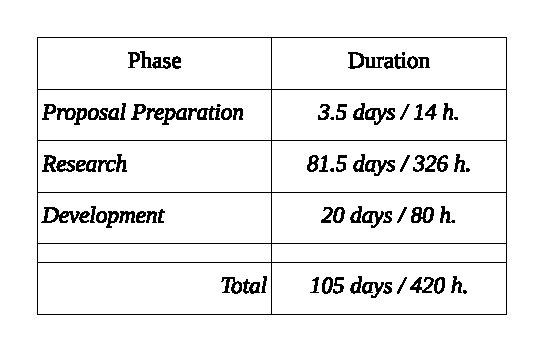
\includegraphics{images/planning-stats.pdf}
\end{table}

\begin{figure}
    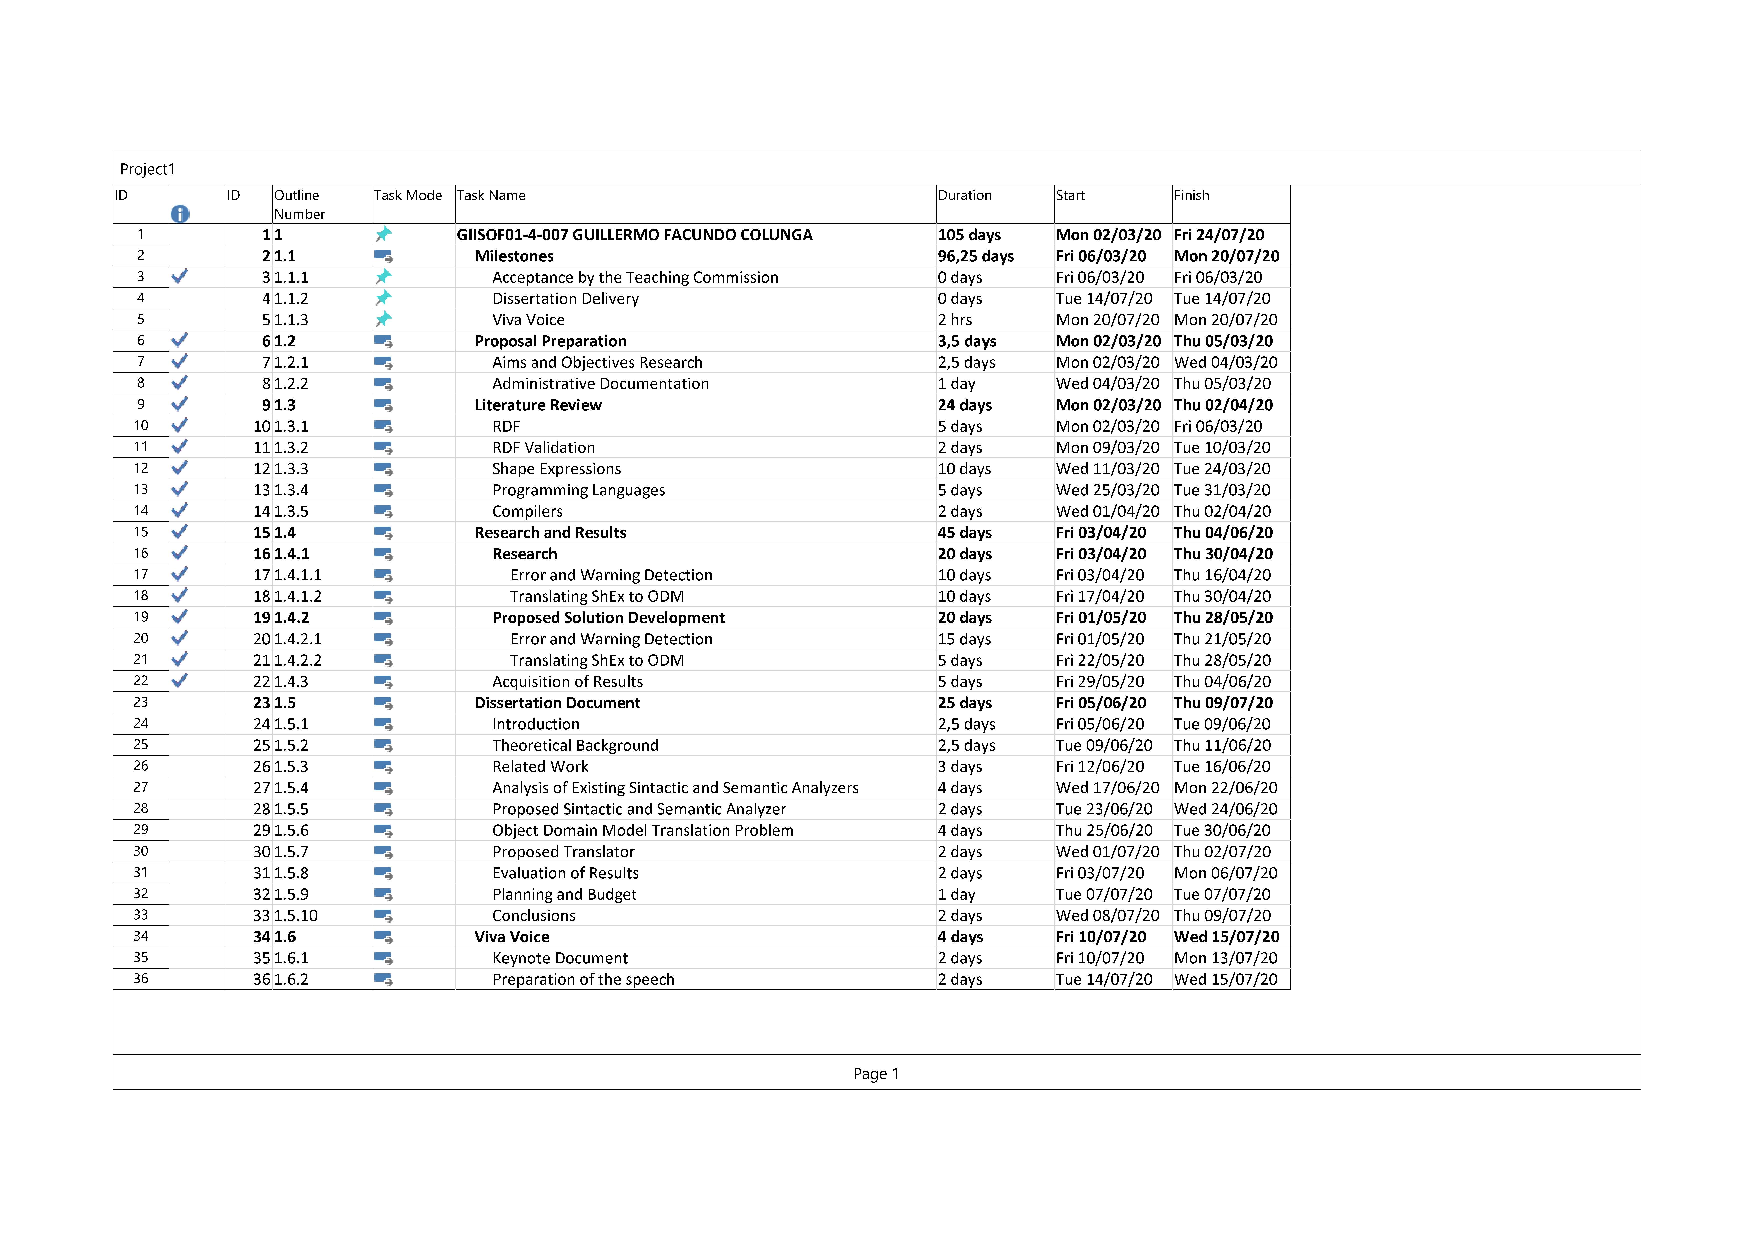
\includegraphics[width=\textwidth]{images/planificacion.pdf}
    \centering
	\caption[Tasks planning of the project]{Tasks planning of the project.}
    \label{fig:planning-sheet}
\end{figure}

\section{Budget}
To calculate this project we will take into account the estimate. From the estimation we can obtain
the time that is dedicated to each of the phases, in addition we have to take into account that not
all tasks are performed by the same profile and therefore not all profiles will have the same remuneration.
	\chapter{Conclusions}
\label{ch:conclusions}

\section{Future Work}
Currently both proposed solutions are based on the reduced ShEx grammar,
therefore the first future work we identify is to be able to bring the philosophies
described in this work to the full ShEx grammar, so that the improvements described
can benefit all users of the language.

The next step would be to expand the range of the static analysis of shape expressions
so that it supports more elements of the grammar so that all the elements that make
up a shape, their dependencies and relationships can be analyzed in much more detail.

	\part{Annexes and References}
	\begin{appendices}
		\chapter{ShEx Micro Language}
		\section{Syntax Specification}
		\section{Lexical Specification}
		\chapter{ShEx-Lite Antlr Grammar}
		\section{Syntax Specification}
		\section{Lexical Specification}
		\chapter{Project Communications}
		\section{Open Source Community}
		\section{Scientific Disclosure}
		\section{Dublin Core Meetings}
	\end{appendices}

	\SgIncludeBib{biblio}
\end{document}